\documentclass[twoside,spanish,a4paper,12pt]{tfg}

% Editar la titulación
\titulacion{Grado en Ingeniería \\ Informática}

% Editar el título
\title{Desarrollo de una tienda online para una droguería}

% Si es una alumna se debe usar
% \authorlabel{Autora}
\authorlabel{Autor}
% Editar el nombre
\author{Carlos Javier Piquer Mañez}


% Si hay varios tutores:
% \tutorlabel{Tutores}
% \tutor{Nombre del tutor 1 \\[2mm] Nombre del turor2}
% Si el tutor es masculino:
% \tutorlabel{Tutor}
\tutorlabel{Tutor}
% Editar
\tutor{Andrés Rocafull Rodrigo} 

% Editar: Poner mes y año de la convocatoria de lectura del TFM
\convocatoria{Junio 2026}

\usepackage{amssymb}
\usepackage{float}
\usepackage{array}
\usepackage{tabularx}
\newcolumntype{L}[1]{>{\raggedright\arraybackslash}p{#1}}
\usepackage{graphicx}  
\usepackage{rotating} 
\usepackage{pdflscape}
\raggedbottom


\begin{document}

% NO QUITAR ESTOS ELEMENTOS
\portada
\cleardoublepage
\contraportada
\cleardoublepage
\declaracion
\cleardoublepage

% Declaración responsable de uso de IA — ETSE-UV
\newpage
\thispagestyle{empty}

\vspace*{4mm}
{\centering
\textbf{\large Declaración responsable de uso de Inteligencia Artificial (IA) — ETSE-UV}\\[4pt]
\small Anexo. Modelo de declaración a adjuntar al TFG/TFM entregado por el alumnado.\\[10mm]
}

\newcommand{\formline}[2][8cm]{\underline{\makebox[#1][l]{\small #2}}}

\noindent\textbf{Yo,} \formline[7.5cm]{Carlos Javier Piquer Mañez} \hfill \textbf{con (NIF/NPA)} \formline[3cm]{23874989T}\\[5mm]
\noindent\textbf{Titulación:} \formline[13cm]{Grado en Ingeniería Informática}\\[5mm]
\noindent\textbf{Título del TFG/TFM:} \formline[11.5cm]{Desarrollo de una tienda online para una droguería}\\[7mm]

\noindent\small Declaro que en este trabajo he utilizado las siguientes herramientas de IA (si procede):\\[3mm]

\noindent 1. Herramienta y versión: \formline[11cm]{Claude Code — Claude Sonnet 4.6 (Anthropic, 2025)}\\[2.5mm]
\noindent 2. Herramienta y versión: \formline[11cm]{Google Gemini 2.5 Pro (Google, 2025)}\\[2.5mm]
\noindent 3. Herramienta y versión: \formline[11cm]{}\\[2.5mm]
\noindent 4. Herramienta y versión: \formline[11cm]{}\\[6mm]
\clearpage
% ---- Helpers para casillas ----
\newcommand{\cbox}{$\boxtimes$}  % marcada
\newcommand{\ubox}{$\square$}    % vacía

% ---- Sección 1 ----
\noindent\textbf{1) Dimensiones de uso de la IA} (marca una opción por fila). Determina el grado de uso de la IA en las siguientes dimensiones.

\smallskip
\noindent\small Escala (5 puntos): 1 = No se ha utilizado IA · 2 = Uso muy puntual · 3 = Uso moderado · 4 = Uso frecuente · 5 = Uso intensivo

\smallskip
\renewcommand{\arraystretch}{1.35}
\begin{tabular}{|p{0.66\textwidth}|c|c|c|c|c|}
\hline
\small\textbf{Dimensión} & \small\textbf{1} & \small\textbf{2} & \small\textbf{3} & \small\textbf{4} & \small\textbf{5} \\
\hline
\small Corrección lingüística: ortografía, gramática, puntuación y coherencia formal del texto
& \ubox & \ubox & \ubox & \ubox & \cbox \\
\hline
\small Reescritura y mejora de estilo: reformulación para aumentar claridad, concisión y legibilidad manteniendo el significado
& \ubox & \ubox & \ubox & \cbox & \ubox \\
\hline
\small Síntesis de contenido: elaboración de resúmenes a partir de textos extensos o complejos para identificar ideas clave
& \ubox & \ubox & \cbox & \ubox & \ubox \\
\hline
\small Apoyo en la localización de referencias: propuesta de posibles fuentes (a verificar y citar correctamente)
& \ubox & \ubox & \ubox & \cbox & \ubox \\
\hline
\small Planificación del trabajo: propuesta de esquemas, índices o guiones iniciales para estructurar el documento
& \ubox & \cbox & \ubox & \ubox & \ubox \\
\hline
\small Mejora de la argumentación y la estructura: detección de huecos, redundancias o saltos lógicos y propuesta de reorganización
& \ubox & \ubox & \cbox & \ubox & \ubox \\
\hline
\small Programación (si procede): apoyo en el desarrollo, depuración u optimización de fragmentos de código puntuales
& \ubox & \ubox & \ubox & \cbox & \ubox \\
\hline
\small Programación (si procede): uso generalizado de herramientas de generación de código de forma autónoma a partir de especificaciones
& \ubox & \ubox & \cbox & \ubox & \ubox \\
\hline
\small Análisis de datos (si procede): ayuda exploratoria para limpieza preliminar, generación de hipótesis e identificación de patrones
& \ubox & \ubox & \ubox & \ubox & \cbox \\
\hline
\small Traducción o adaptación lingüística (si procede)
& \cbox & \ubox & \ubox & \ubox & \ubox \\
\hline
\small Soporte en material visual (si procede): ideas para figuras, tablas o gráficos y revisión de su explicación
& \ubox & \ubox & \ubox & \cbox & \ubox \\
\hline
\small Otros (especificar): \underline{\hspace{6cm}}
& \ubox & \ubox & \ubox & \ubox & \ubox \\
\hline
\end{tabular}

\bigskip

% ---- Sección 2 ----
\noindent\textbf{2) Compromisos de uso responsable} (marca tu grado de acuerdo). Determina si se ha realizado un uso responsable de la IA.

\smallskip
\noindent\small Escala (acuerdo): 1 = Totalmente en desacuerdo · 2 = En desacuerdo · 3 = Neutral · 4 = De acuerdo · 5 = Totalmente de acuerdo

\smallskip
\begin{tabular}{|p{0.66\textwidth}|c|c|c|c|c|}
\hline
\small\textbf{Declaración} & \small\textbf{1} & \small\textbf{2} & \small\textbf{3} & \small\textbf{4} & \small\textbf{5} \\
\hline
\small Las ideas principales, interpretaciones y análisis críticos del trabajo son propios.
& \ubox & \ubox & \ubox & \ubox & \cbox \\
\hline
\small El uso de IA no ha sustituido mis competencias básicas de investigación, redacción y razonamiento académico.
& \ubox & \ubox & \ubox & \ubox & \cbox \\
\hline
\small He revisado, contrastado e integrado críticamente cualquier contenido generado con IA antes de incorporarlo.
& \ubox & \ubox & \ubox & \ubox & \cbox \\
\hline
\small He verificado la precisión y fiabilidad del contenido, incluyendo datos, afirmaciones y referencias bibliográficas.
& \ubox & \ubox & \ubox & \cbox & \ubox \\
\hline
\end{tabular}

\bigskip
\clearpage
\noindent\textbf{Observaciones (opcional)}

\smallskip
\noindent\rule{\textwidth}{0.4pt}

\bigskip\bigskip

\noindent\small A través de esta declaración, afirmo que he descrito de manera transparente y fidedigna el uso de IA de este trabajo. Asumo la autoría y responsabilidad de la obra final y confirmo que no he introducido datos personales o confidenciales contraviniendo la normativa de protección de datos personales\footnote{Ley orgánica 3/2018, de 5 de diciembre, de protección de datos personales y garantía de los derechos digitales.} y que he respetado las normas en materia de propiedad intelectual\footnote{Ley de propiedad intelectual: Real Decreto Legislativo 1/1996, de 12 de abril.}, así como las previsiones sobre integridad académica\footnote{Código de Convivencia y Buenas Prácticas (ACGUV 300/2023).} de la Universitat de València.

\bigskip\bigskip

\noindent Fecha: \underline{\makebox[1.2cm][c]{19}} / \underline{\makebox[1.2cm][c]{06}} / \underline{\makebox[1.8cm][c]{2026}} \hfill Firma: \raisebox{-0.6cm}{
\includegraphics[height=1.8cm, trim=200 150 100 150, clip]{figs/firma}}

\cleardoublepage

% Editar: Resumen en Español (obligatorio)
\begin{resumen}
El presente trabajo describe el desarrollo de una tienda online completa para la Droguería Mercería Inés, un negocio familiar ubicado en Valencia. La solución implementa el flujo íntegro de comercio electrónico: registro y autenticación de usuarios, catálogo de productos con filtros y buscador, gestión del carrito, pagos seguros mediante la pasarela \textit{Stripe} y generación automática de facturas en PDF. El sistema incorpora además un panel de administración para la gestión del inventario y el seguimiento de pedidos, así como un \textit{bot de Telegram} que automatiza las notificaciones de confirmación de compra y los avisos de bajo stock.

La arquitectura se fundamenta en \textbf{Angular} para el \textit{frontend}, \textbf{Spring Boot} para el \textit{backend} y \textbf{MySQL} como sistema de gestión de base de datos. Todas las herramientas empleadas son gratuitas y de código abierto, lo que hace viable la solución tanto en entornos académicos como en pequeñas empresas.

El resultado es una aplicación web funcional y completa que cubre las necesidades reales del negocio, validada mediante pruebas funcionales, de rendimiento y de usabilidad.
\end{resumen}
\cleardoublepage

% Editar: Resumen en Inglés
\begin{abstract}
This project describes the development of a complete online store for Droguería Mercería Inés, a family business located in Valencia, Spain. The solution implements the full e-commerce workflow: user registration and authentication, a product catalogue with filters and search, shopping cart management, secure payments through the \textit{Stripe} gateway, and automatic PDF invoice generation. The system also includes an administration panel for inventory management and order tracking, as well as a \textit{Telegram bot} that automates purchase confirmation notifications and low-stock alerts.

The architecture is built on \textbf{Angular} for the frontend, \textbf{Spring Boot} for the backend, and \textbf{MySQL} as the database management system. All tools used are free and open source, making the solution viable for both academic and small-business environments.

The result is a fully functional web application that meets the real needs of the business, validated through functional, performance, and usability testing.
\end{abstract}
\cleardoublepage

% Editar: Resumen en Valenciano
\begin{resum}
Aquest treball descriu el desenvolupament d'una botiga en línia completa per a la Drogueria Merceria Inés, un negoci familiar ubicat a València. La solució implementa el flux complet de comerç electrònic: registre i autenticació d'usuaris, catàleg de productes amb filtres i cercador, gestió del carret, pagaments segurs mitjançant la passarel·la \textit{Stripe} i generació automàtica de factures en PDF. El sistema incorpora també un panell d'administració per a la gestió de l'inventari i el seguiment de les comandes, així com un \textit{bot de Telegram} que automatitza les notificacions de confirmació de compra i els avisos de baix estoc.

L'arquitectura es fonamenta en \textbf{Angular} per al \textit{frontend}, \textbf{Spring Boot} per al \textit{backend} i \textbf{MySQL} com a sistema de gestió de base de dades. Totes les eines emprades són gratuïtes i de codi obert, la qual cosa fa viable la solució tant en entorns acadèmics com en xicotetes empreses.

El resultat és una aplicació web funcional i completa que cobreix les necessitats reals del negoci, validada mitjançant proves funcionals, de rendiment i d'usabilitat.
\end{resum}
\cleardoublepage


% Editar: Agradecimientos (opcional)
\begin{agradecimientos}
  En primer lugar quiero agradecer a todos aquellos que me han apoyado durante todos estos años.

  En segundo lugar...
\end{agradecimientos}
\cleardoublepage

\tableofcontents

\pagestyle{tfg}
\justify

% Las figuras se buscan en el directorio figs

% Cada capítulo está en su propio fichero tex. Ver el directorio tex.

% La bibliografía está dentro del directorio bib
\chapter{Introducción}
% Contenidos del capítulo.
% Las secciones presentadas son orientativas y no representan
% necesariamente la organización que debe tener este capítulo.

\section{Introducción}

El presente trabajo de fin de grado describe el desarrollo de una \textbf{tienda online} para la \textbf{Droguería Mercería Inés}, un negocio familiar ubicado en Valencia. El establecimiento, regentado por Ester, ofrece una amplia variedad de productos: perfumes, utensilios de costura, hilos, telas especiales y artículos de mercería en general, siguiendo la tradición de las droguerías de barrio que durante décadas han formado parte del comercio local.

Aunque el negocio cuenta con presencia en redes sociales, no disponía de una página web propia que permitiese a sus clientes consultar el catálogo, realizar pedidos y efectuar pagos de forma online. Este proyecto nace con el objetivo de cubrir esa necesidad mediante el desarrollo de una aplicación web completa, construida íntegramente con herramientas gratuitas y de código abierto.

La solución desarrollada permite a los clientes registrarse, explorar el catálogo de productos, gestionar su carrito y completar compras a través de la pasarela de pago \textit{Stripe}. Por parte de la administración, el sistema facilita la gestión del inventario y el seguimiento de pedidos, con notificaciones automáticas de confirmación de compra y avisos de bajo stock a través de un \textit{bot de Telegram}.

\section{Motivación}

La principal motivación de este proyecto es de carácter personal: dar respuesta a una necesidad real de un negocio familiar. La Droguería Mercería Inés tiene presencia en redes sociales, pero carecía de una plataforma web propia desde la que sus clientes pudieran realizar compras de manera cómoda y segura. Desarrollar esta solución supone una aportación directa al negocio de la familia, facilitando tanto la experiencia de compra de los clientes como el trabajo diario de la propietaria en la gestión del stock y los pedidos.

Además, existe una motivación de carácter profesional. La elección de \textbf{Angular} y \textbf{Spring Boot} como tecnologías principales responde al hecho de que son las herramientas utilizadas en \textbf{Capgemini}, empresa en la que se van a realizar las prácticas. Abordar este proyecto ha permitido adquirir una base sólida en ambas tecnologías antes de incorporarse a un entorno profesional, complementando la formación académica con una experiencia de desarrollo real y completa.

Por último, este proyecto pretende demostrar que es posible construir una solución de comercio electrónico funcional y profesional haciendo uso exclusivamente de herramientas \textbf{gratuitas y de código abierto}, sin necesidad de recurrir a plataformas de pago ni a infraestructuras costosas.

\section{Objetivos}

El objetivo principal del proyecto es el siguiente:

\begin{itemize}
    \item \textbf{Desarrollar una tienda online funcional y completa para la Droguería Mercería Inés}, que permita a sus clientes consultar el catálogo, realizar pedidos y efectuar pagos de forma segura a través de internet.
\end{itemize}

Para alcanzarlo, se han definido los siguientes objetivos secundarios:

\begin{itemize}
    \item Dar visibilidad online al negocio mediante una plataforma web propia, complementando su presencia actual en redes sociales.
    \item Facilitar a la propietaria el control del inventario y el seguimiento de los pedidos recibidos a través de la aplicación.
    \item Automatizar las notificaciones de confirmación de pedido y los avisos de bajo stock mediante un bot de Telegram integrado en el sistema.
    \item Adquirir experiencia práctica en \textbf{Angular} y \textbf{Spring Boot} como preparación para las prácticas profesionales en Capgemini.
    \item Demostrar que una solución de comercio electrónico completa puede desarrollarse íntegramente con herramientas gratuitas y de código abierto.
\end{itemize}

\section{Organización de la memoria}

La memoria se organiza en los siguientes capítulos:

\begin{itemize}
    \item \textbf{Capítulo 1 — Introducción:} presenta el proyecto, su motivación, los objetivos planteados y la estructura del documento.
    \item \textbf{Capítulo 2 — Estado del arte:} analiza las plataformas de creación de tiendas online más representativas y estudia las tecnologías seleccionadas para el desarrollo del sistema, justificando cada elección.
    \item \textbf{Capítulo 3 — Requisitos, especificaciones, coste, riesgos y viabilidad:} recoge los requisitos funcionales y no funcionales del sistema, las especificaciones técnicas, la planificación temporal y económica del proyecto, los riesgos identificados y el análisis de viabilidad.
    \item \textbf{Capítulo 4 — Análisis:} incluye los diagramas de análisis del sistema: el diagrama de casos de uso, el diagrama de clases de análisis y los diagramas de secuencia general del sistema (DSGS).
    \item \textbf{Capítulo 5 — Diseño:} describe la arquitectura general del sistema, los diagramas UML de diseño, el modelo de la base de datos y los prototipos de la interfaz de usuario.
    \item \textbf{Capítulo 6 — Implementación y pruebas:} detalla el proceso de desarrollo de la aplicación y los resultados de las pruebas funcionales, de rendimiento y de usabilidad realizadas.
    \item \textbf{Capítulo 7 — Conclusiones:} revisa los costes finales del proyecto, presenta las conclusiones obtenidas y propone posibles líneas de trabajo futuro.
\end{itemize}


\chapter{Estado del arte}
% ======================================
% CAPÍTULO 2 - ESTADO DEL ARTE
% ======================================

\section{Análisis de aplicaciones similares}
En el mercado actual la gran variedad de plataformas que nos ofrecen servicios para
crear nuestra propia tienda online sin necesidad de tener algún tipo de conocimiento sobre
programar es muy extenso. Algunas de las más representativas son:

\subsection{Wix eCommerce}
Wix proporciona un sistema de creación de páginas basado en el uso de herramientas
de arrastrar y soltar, lo que facilita a cualquier usuario construir una tienda en poco
tiempo \cite{wixHelp}. Sin embargo, esta simplicidad también conlleva limitaciones, especialmente en lo
que respecta a la personalización avanzada y al control sobre el backend, aspectos que resultan esenciales en proyectos con requisitos específicos.

\textbf{Ventajas:}
\begin{itemize}
    \item Interfaz intuitiva y sistema de diseño drag-and-drop.
    \item Plantillas atractivas y actualizadas.
    \item Incluye hosting y mantenimiento automático.
    \item Integración sencilla con herramientas externas.
\end{itemize}

\textbf{Desventajas:}
\begin{itemize}
    \item Escasa flexibilidad para personalizaciones complejas.
    \item Limitaciones en el acceso al código fuente.
    \item Dificultades para escalar proyectos grandes.
    \item Dependencia total del ecosistema de Wix.
\end{itemize}

\subsection{Squarespace}
Squarespace está orientado a usuarios que priorizan el diseño visual y la facilidad de
uso \cite{squarespaceHelp}. Sus plantillas resultan intuitivas y permiten crear páginas atractivas sin dificultad. No
obstante, su ecosistema de integraciones es más limitado, lo que restringe su aplicabilidad
en proyectos que requieren funcionalidades técnicas más avanzadas.

\textbf{Ventajas:}
\begin{itemize}
    \item Excelente diseño visual y acabados profesionales.
    \item Plataforma todo en uno (hosting, dominio y soporte).
    \item Adaptación automática a dispositivos móviles.
    \item Seguridad gestionada por la propia plataforma.
\end{itemize}

\textbf{Desventajas:}
\begin{itemize}
    \item Pocas integraciones con APIs o sistemas externos.
    \item Costes mensuales relativamente altos.
    \item Escasa libertad para modificar la estructura del sitio.
    \item Dependencia del entorno cerrado de Squarespace.
\end{itemize}

\subsection{PrestaShop}
PrestaShop es una solución de código abierto muy popular para la creación de tiendas
online \cite{prestashopDocs}. Ofrece una gran capacidad de personalización mediante módulos y plantillas, lo que la convierte en una opción atractiva para pequeñas y medianas empresas. No obstante, requiere ciertos conocimientos técnicos para su instalación y mantenimiento, y en proyectos de mayor tamaño puede presentar dificultades de rendimiento si no se configura correctamente.

\textbf{Ventajas:}
\begin{itemize}
    \item Open source y altamente personalizable.
    \item Gran comunidad de desarrolladores.
    \item Amplio catálogo de módulos y temas.
    \item Permite control total sobre el servidor y la base de datos.
\end{itemize}

\textbf{Desventajas:}
\begin{itemize}
    \item Necesita conocimientos técnicos para instalación y soporte.
    \item Requiere mantenimiento y actualizaciones manuales.
    \item Puede presentar problemas de rendimiento en tiendas grandes.
    \item Algunos módulos son de pago y elevan los costes.
\end{itemize}

\subsection{Comparación con la propuesta del TFG}
Las plataformas analizadas muestran distintas formas de crear una tienda online sin necesidad de conocimientos de programación. Wix y Squarespace destacan por su sencillez
y diseño intuitivo, aunque sacrifican flexibilidad y control sobre la aplicación. Por su parte, PrestaShop ofrece mayor capacidad de personalización, pero exige un nivel técnico más elevado y puede presentar limitaciones de rendimiento en proyectos de gran escala.
En contraste, la propuesta de este TFG plantea el desarrollo de una solución a medida  que permita un mayor control sobre la arquitectura, la seguridad y las integraciones, 
adaptándose específicamente a las necesidades del proyecto.


\begin{table}[H]
\centering
\begin{tabular}{|l|c|c|c|}
\hline
\textbf{Criterio} & \textbf{Wix} & \textbf{Squarespace} & \textbf{PrestaShop} \\ \hline
Facilidad de uso & Muy alta & Alta & Media \\ \hline
Personalización & Baja & Media & Alta \\ \hline
Escalabilidad & Limitada & Media & Alta \\ \hline
Requiere conocimientos técnicos & No & No & Sí \\ \hline
Coste & Medio & Medio & Variable \\ \hline
\end{tabular}
\caption{Comparativa de plataformas de creación de tiendas online}
\end{table}


\section{Tecnologías}

\subsection{Frameworks frontend}

\subsubsection{Angular}
Angular es un framework desarrollado por Google y basado en TypeScript \cite{angularDocs}. Ofrece una solución completa para el desarrollo de aplicaciones web a gran escala, con herramientas integradas como enrutamiento y gestión de formularios. Su principal desventaja es la necesidad de contar con conocimientos previos más avanzados, lo que incrementa la curva de aprendizaje.

\textbf{Ventajas:}
\begin{itemize}
    \item Framework completo con soporte oficial de Google.
    \item Tipado fuerte con TypeScript, que mejora la robustez del código.
    \item Soporte integrado para testing, formularios y enrutamiento.
    \item Comunidad amplia y documentación exhaustiva.
\end{itemize}

\textbf{Desventajas:}
\begin{itemize}
    \item Curva de aprendizaje pronunciada.
    \item Tamaño inicial del proyecto elevado.
    \item Requiere experiencia previa en TypeScript.
    \item Sintaxis más compleja frente a otras alternativas.
\end{itemize}

\subsubsection{React}
React es una tecnología desarrollada por Meta \cite{reactDocs}. Se trata de una biblioteca para la construcción de interfaces de usuario, que destaca por su flexibilidad y por el rendimiento que ofrece gracias al uso del Virtual DOM. Sin embargo, al no ser un framework completo, depende de librerías de la comunidad para cubrir funcionalidades adicionales o más avanzadas.

\textbf{Ventajas:}
\begin{itemize}
    \item Excelente rendimiento gracias al Virtual DOM.
    \item Gran comunidad y recursos de aprendizaje.
    \item Compatible con múltiples librerías y frameworks.
    \item Curva de aprendizaje accesible para principiantes.
\end{itemize}

\textbf{Desventajas:}
\begin{itemize}
    \item Necesidad de integrar herramientas externas (routing, estado).
    \item Menor estructura definida que Angular.
    \item Frecuentes actualizaciones y cambios en librerías.
    \item Requiere experiencia para mantener proyectos grandes.
\end{itemize}

\subsubsection{Vue}
Vue es un framework progresivo creado por Evan You, exingeniero de Google \cite{vueDocs}. Combina características de Angular y React, con un enfoque en la simplicidad y en la rapidez de aprendizaje. No obstante, su comunidad y ecosistema siguen siendo más reducidos en comparación con otras tecnologías consolidadas.

\textbf{Ventajas:}
\begin{itemize}
    \item Ligero y de fácil adopción.
    \item Documentación clara y organizada.
    \item Buena integración con proyectos existentes.
    \item Sintaxis sencilla y curva de aprendizaje rápida.
\end{itemize}

\textbf{Desventajas:}
\begin{itemize}
    \item Ecosistema más limitado que Angular o React.
    \item Menor presencia en grandes empresas.
    \item Menos recursos de formación avanzada.
    \item Riesgo de menor soporte a largo plazo.
\end{itemize}

\subsubsection{Comparación y elección}
Los tres frameworks permiten crear aplicaciones modernas, pero Angular ofrece una
estructura más completa desde el inicio. Para este TFG se ha optado por Angular, ya que
es la tecnología utilizada en Capgemini, empresa en la que se van a realizar las prácticas. De
esta forma, el proyecto servirá también como una preparación práctica, complementada
con cursos de formación, para no comenzar esa experiencia sin conocimientos previos.

\begin{table}[H]
\centering
\begin{tabular}{|l|c|c|c|}
\hline
\textbf{Criterio} & \textbf{Angular} & \textbf{React} & \textbf{Vue} \\ \hline
Lenguaje principal & TypeScript & JavaScript & JavaScript \\ \hline
Complejidad inicial & Alta & Media & Baja \\ \hline
Ecosistema & Muy amplio & Amplio & Moderado \\ \hline
Soporte empresarial & Alto & Alto & Medio \\ \hline
Rendimiento general & Alto & Muy alto & Alto \\ \hline
\end{tabular}
\caption{Comparativa de frameworks frontend}
\end{table}


\subsection{Frameworks backend}

\subsubsection{Spring Boot}
Spring Boot es un framework del ecosistema Java que facilita la creación de aplicaciones backend robustas y escalables \cite{springDocs}. Entre sus principales ventajas se encuentran su amplia comunidad, la integración con múltiples librerías y la facilidad para configurar proyectos complejos. Como inconvenientes, requiere conocimientos previos en Java y, según el tamaño de la aplicación, puede resultar más pesado que otras alternativas.

\textbf{Ventajas:}
\begin{itemize}
    \item Framework maduro con gran soporte empresarial.
    \item Integración nativa con bases de datos y APIs REST.
    \item Facilita pruebas y despliegues automáticos.
    \item Gran estabilidad y seguridad.
\end{itemize}

\textbf{Desventajas:}
\begin{itemize}
    \item Requiere conocimientos avanzados en Java.
    \item Consumo de recursos más alto que Node.js.
    \item Curva de aprendizaje larga.
    \item Configuraciones iniciales complejas.
\end{itemize}

\subsubsection{Node.js}
Node.js es un entorno de ejecución de JavaScript que permite utilizar este lenguaje en la configuración y desarrollo de servidores \cite{nodeDocs}. Destaca por su rendimiento en aplicaciones en tiempo real y por la ventaja de compartir el mismo lenguaje en frontend y backend, lo que agiliza el desarrollo. Su principal limitación es que no está tan orientado a aplicaciones de gran escala como otros frameworks más consolidados.

\textbf{Ventajas:}
\begin{itemize}
    \item Excelente rendimiento en tiempo real.
    \item Usa el mismo lenguaje en cliente y servidor.
    \item Amplia comunidad y soporte.
    \item Ecosistema extenso con NPM.
\end{itemize}

\textbf{Desventajas:}
\begin{itemize}
    \item Menor rendimiento en tareas muy pesadas.
    \item Dificultad para proyectos altamente estructurados.
    \item Depende mucho de librerías externas.
    \item Escalabilidad más limitada que Spring Boot.
\end{itemize}

\subsubsection{Django}
Django es un framework de Python que sigue el principio "batteries included", lo que significa que incorpora numerosas funcionalidades listas para usar \cite{djangoDocs}. Es adecuado para el desarrollo rápido de prototipos y proyectos de tamaño medio, con una curva de aprendizaje moderada. Sin embargo, su rendimiento puede verse limitado en aplicaciones muy exigentes.

\textbf{Ventajas:}
\begin{itemize}
    \item Gran cantidad de herramientas integradas.
    \item Excelente para desarrollo rápido.
    \item Seguridad y control de autenticación robusto.
    \item Documentación muy completa.
\end{itemize}

\textbf{Desventajas:}
\begin{itemize}
    \item Menor rendimiento en aplicaciones grandes.
    \item Menor integración con sistemas Java.
    \item No tan extendido en entornos empresariales.
    \item Difícil de optimizar para proyectos complejos.
\end{itemize}

\subsubsection{Comparación y elección}
Spring Boot, Node.js y Django son alternativas viables para el desarrollo de un backend. Node.js destaca por su rapidez en tiempo real y Django por la simplicidad de Python, pero para este TFG se ha optado por Spring Boot. Esta elección responde a que es la tecnología utilizada en Capgemini, empresa en la que se realizarán las prácticas, lo
que permite formarse previamente mediante cursos y adquirir los conceptos básicos necesarios. Además, Spring Boot destaca por su robustez, su madurez en entornos empresariales y porque complementa de forma óptima la arquitectura planteada con Angular y SQL.

\begin{table}[H]
\centering
\begin{tabular}{|l|c|c|c|}
\hline
\textbf{Criterio} & \textbf{Spring Boot} & \textbf{Node.js} & \textbf{Django} \\ \hline
Lenguaje base & Java & JavaScript & Python \\ \hline
Escalabilidad & Alta & Media & Media \\ \hline
Curva de aprendizaje & Alta & Media & Baja \\ \hline
Rendimiento general & Alto & Alto & Medio \\ \hline
Soporte empresarial & Muy alto & Medio & Medio \\ \hline
\end{tabular}
\caption{Comparativa de frameworks backend}
\end{table}


\subsection{Bots de Telegram}

Los bots de Telegram son programas automatizados que interactúan con usuarios a través de la plataforma de mensajería Telegram mediante su API oficial. Permiten enviar notificaciones, gestionar comandos y ejecutar acciones en respuesta a eventos externos, lo que los convierte en una alternativa práctica para integrar comunicaciones automatizadas en aplicaciones web. A continuación se analizan las principales librerías disponibles para su desarrollo.

\subsubsection{python-telegram-bot}
python-telegram-bot es una librería de código abierto escrita en Python que proporciona una interfaz completa para interactuar con la API oficial de Telegram \cite{pythonTelegramBotDocs}. Ofrece soporte tanto para \textit{polling} como para \textit{webhooks}, y su diseño basado en \textit{handlers} facilita la estructuración del código. Sin embargo, al estar escrita en Python, su integración con proyectos Java como Spring Boot requiere desplegar un servicio adicional.

\textbf{Ventajas:}
\begin{itemize}
    \item Librería madura y bien documentada.
    \item Soporte completo para la API de Telegram.
    \item Gran comunidad activa y amplia cantidad de ejemplos.
    \item Compatible con \textit{polling} y \textit{webhooks}.
\end{itemize}

\textbf{Desventajas:}
\begin{itemize}
    \item Requiere un servicio Python independiente si el backend es Java.
    \item Mayor complejidad de despliegue en proyectos políglotas.
    \item Gestión de dependencias separada del proyecto principal.
    \item Puede presentar latencias si no se configura correctamente el \textit{webhook}.
\end{itemize}

\subsubsection{Telegraf}
Telegraf es un framework moderno para el desarrollo de bots de Telegram basado en Node.js y TypeScript \cite{telegrafDocs}. Destaca por su arquitectura orientada a \textit{middleware} y su sintaxis clara y expresiva, lo que facilita la creación de bots complejos con pocas líneas de código. Al igual que python-telegram-bot, requiere un entorno de ejecución independiente cuando se combina con un backend Java.

\textbf{Ventajas:}
\begin{itemize}
    \item Sintaxis moderna y expresiva basada en \textit{middleware}.
    \item Soporte nativo para TypeScript.
    \item Amplio ecosistema de plugins y extensiones.
    \item Buena documentación y comunidad activa.
\end{itemize}

\textbf{Desventajas:}
\begin{itemize}
    \item Requiere entorno Node.js separado del backend Java.
    \item Curva de aprendizaje mayor si no se tiene experiencia con Node.js.
    \item Dependencia del ecosistema NPM.
    \item Configuración adicional para despliegues en producción.
\end{itemize}

\subsubsection{TelegramBots (Java)}
TelegramBots es una librería Java de código abierto que implementa la API de Telegram directamente en el ecosistema Java \cite{telegramBotsDocs}. Su integración nativa con Spring Boot permite incorporar el bot dentro del mismo proyecto sin necesidad de servicios adicionales, simplificando el despliegue y el mantenimiento. Es la opción más coherente para proyectos backend basados en Java.

\textbf{Ventajas:}
\begin{itemize}
    \item Integración directa con Spring Boot sin servicios adicionales.
    \item Mismo lenguaje y entorno que el resto del backend.
    \item Soporte completo para la API de Telegram.
    \item Simplifica el despliegue al unificar bot y backend en un solo proyecto.
\end{itemize}

\textbf{Desventajas:}
\begin{itemize}
    \item Comunidad más reducida que las alternativas en Python o Node.js.
    \item Documentación menos extensa en comparación con python-telegram-bot.
    \item Menor cantidad de ejemplos y recursos de aprendizaje.
    \item Actualizaciones menos frecuentes que otras librerías.
\end{itemize}

\subsubsection{Comparación y elección}
Las tres opciones analizadas permiten desarrollar bots funcionales para Telegram, pero difieren en el lenguaje y el entorno de ejecución requerido. python-telegram-bot y Telegraf destacan por su popularidad y documentación, aunque ambas necesitan un servicio independiente cuando el backend está desarrollado en Java. Para este TFG se ha optado por \textbf{TelegramBots (Java)} por su integración nativa con Spring Boot, lo que permite incorporar el bot directamente en el mismo proyecto sin añadir complejidad de despliegue. Esta elección mantiene la coherencia tecnológica de la arquitectura y facilita el mantenimiento del sistema.

\begin{table}[H]
\centering
\resizebox{\textwidth}{!}{%
\begin{tabular}{|l|c|c|c|}
\hline
\textbf{Criterio} & \textbf{python-telegram-bot} & \textbf{Telegraf} & \textbf{TelegramBots (Java)} \\ \hline
Lenguaje & Python & Node.js / TypeScript & Java \\ \hline
Integración con Spring Boot & Indirecta & Indirecta & Nativa \\ \hline
Facilidad de uso & Alta & Alta & Media \\ \hline
Documentación & Muy completa & Completa & Limitada \\ \hline
Despliegue en proyecto Java & Complejo & Complejo & Simple \\ \hline
\end{tabular}%
}
\caption{Comparativa de librerías para bots de Telegram}
\end{table}


\subsection{Bases de datos}

\subsubsection{SQL}
Las bases de datos relacionales, como MySQL o PostgreSQL, utilizan un modelo basado en tablas y relaciones entre ellas \cite{mysqlDocs}. Destacan por su consistencia, su alto nivel de seguridad y por el uso del lenguaje SQL, que es un estándar ampliamente adoptado en el entorno empresarial.

\subsubsection{NoSQL}
Las bases de datos NoSQL, como MongoDB, almacenan la información en estructuras más flexibles, como documentos o grafos. Ofrecen mayor escalabilidad y rapidez en ciertas operaciones, aunque sacrifican consistencia y mecanismos de seguridad más avanzados. \cite{mongodbDocs}.

\subsubsection{Comparación y elección}
Para este TFG se ha optado por utilizar \textbf{MySQL} como sistema de gestión de bases de datos. La elección se debe a su estabilidad, su integración nativa con Spring Boot y su capacidad para garantizar la seguridad de los datos. Además, a lo largo de la carrera se ha trabajado ampliamente con bases de datos SQL, mientras que NoSQL apenas se ha tratado, por lo que MySQL resulta una opción más familiar y adecuada para el desarrollo del proyecto.

\begin{table}[H]
\centering
\begin{tabular}{|l|c|c|}
\hline
\textbf{Criterio} & \textbf{SQL (MySQL)} & \textbf{NoSQL (MongoDB)} \\ \hline
Estructura & Tablas relacionales & Documentos / grafos \\ \hline
Consistencia & Alta & Media \\ \hline
Seguridad & Alta & Media \\ \hline
Escalabilidad & Media & Alta \\ \hline
Soporte empresarial & Muy alto & Medio \\ \hline
\end{tabular}
\caption{Comparativa entre bases de datos SQL y NoSQL}
\end{table}

\subsection{Pasarelas de pago}

\subsubsection{PayPal}
PayPal es una de las plataformas de pago online más conocidas y utilizadas a nivel mundial \cite{paypalDocs}. Permite realizar transacciones de forma sencilla y segura, tanto con tarjeta como con saldo en cuenta. Es muy popular entre los usuarios por su rapidez y confianza, aunque cobra comisiones algo más altas que otras alternativas.

\textbf{Ventajas:}
\begin{itemize}
    \item Gran confianza y reconocimiento internacional.
    \item Permite pagar sin necesidad de introducir datos bancarios en cada compra.
    \item Interfaz sencilla para el usuario.
    \item Compatible con muchas plataformas de comercio electrónico.
\end{itemize}

\textbf{Desventajas:}
\begin{itemize}
    \item Comisiones elevadas por transacción.
    \item Poca flexibilidad para personalizar el flujo de pago.
    \item Integración técnica menos avanzada que otras opciones.
    \item Posibles retenciones temporales de fondos en algunas operaciones.
\end{itemize}


\subsubsection{Redsys}
Redsys es la pasarela de pago más extendida en España y se utiliza en la mayoría de tiendas online que trabajan con bancos nacionales \cite{redsysDocs}. Ofrece un alto nivel de seguridad y cumple con las normativas europeas, aunque su configuración inicial puede ser más compleja y su documentación menos accesible para desarrolladores.

\textbf{Ventajas:}
\begin{itemize}
    \item Muy utilizada en España, con soporte por parte de los principales bancos.
    \item Alta seguridad gracias al uso de sistemas 3D Secure.
    \item Cumple con las normativas PSD2 y SCA.
    \item Fiable y con buena reputación en entornos comerciales.
\end{itemize}

\textbf{Desventajas:}
\begin{itemize}
    \item Configuración inicial compleja.
    \item Documentación técnica limitada.
    \item Poco orientada a desarrolladores.
    \item Limitada flexibilidad en integraciones personalizadas.
\end{itemize}


\subsubsection{Stripe}
Stripe es una pasarela de pago moderna pensada especialmente para desarrolladores \cite{stripeDocs}. Su API es clara y bien documentada, lo que facilita mucho la integración con aplicaciones web. Permite gestionar pagos con tarjeta, transferencias y otros métodos de forma segura y rápida. Es una opción muy utilizada por startups y empresas tecnológicas por su facilidad de uso y sus amplias posibilidades de personalización.

\textbf{Ventajas:}
\begin{itemize}
    \item API muy completa y fácil de integrar.
    \item Admite múltiples métodos de pago y divisas.
    \item Buen equilibrio entre seguridad y personalización.
    \item Excelente documentación y comunidad activa.
\end{itemize}

\textbf{Desventajas:}
\begin{itemize}
    \item Requiere conocimientos técnicos básicos para la configuración.
    \item Comisiones similares a las de PayPal.
    \item Depende de una conexión estable con la API.
    \item No disponible en todos los países.
\end{itemize}


\subsubsection{Comparación y elección}
PayPal, Redsys y Stripe son tres opciones válidas para integrar pagos en una tienda online. PayPal destaca por su popularidad y facilidad de uso, mientras que Redsys es la alternativa más común en España y ofrece gran seguridad. Sin embargo, para este TFG se ha optado por \textbf{Stripe} debido a su flexibilidad, buena documentación y facilidad de integración con tecnologías modernas como Spring Boot y Angular. Además, su API REST simplifica la conexión con el backend y garantiza un proceso de pago seguro y fluido para el usuario.

\begin{table}[H]
\centering
\begin{tabular}{|l|c|c|c|}
\hline
\textbf{Criterio} & \textbf{PayPal} & \textbf{Redsys} & \textbf{Stripe} \\ \hline
Popularidad & Muy alta & Alta & Alta \\ \hline
Facilidad de integración & Media & Baja & Alta \\ \hline
Comisiones & Altas & Medias & Medias \\ \hline
Orientación a desarrolladores & Baja & Baja & Muy alta \\ \hline
Seguridad & Alta & Muy alta & Alta \\ \hline
\end{tabular}
\caption{Comparativa de pasarelas de pago}
\end{table}




\chapter{Requisitos, especificaciones, coste, riesgos, viabilidad}
% Contenidos del capítulo
% Las secciones presentadas son orientativas y no representan
% necesariamente la organización que debe tener este capítulo.
% =============================
% Capítulo 3: Requisitos, especificaciones, coste, riesgos y viabilidad
% =============================
En este capítulo se presenta un estudio inicial del proyecto, analizando los requisitos, especificaciones, costes, riesgos y viabilidad del sistema desarrollado. 
El objetivo es definir las \textbf{funcionalidades necesarias} para el correcto funcionamiento de la aplicación, detallar sus \textbf{especificaciones técnicas}, estimar el \textbf{coste y el tiempo de desarrollo}, identificar los \textbf{principales riesgos} y, finalmente, valorar la \textbf{viabilidad global} del proyecto. A continuación, se detallan los distintos apartados que conforman este estudio.

% Requisitos del sistema
\section{Requisitos}

El sistema propuesto consiste en una \textbf{plataforma web de comercio electrónico para una droguería} que permite a los usuarios registrarse, explorar productos, filtrar resultados, gestionar su carrito de compra, realizar pagos mediante un servicio externo (Stripe) y recibir notificaciones automáticas mediante el bot de Telegram. 
Por parte del administrador, el sistema debe permitir filtrar pedidos, añadir productos, así como consultar y modificar los pedidos existentes.

A continuación, se detallan los requisitos funcionales y no funcionales definidos para el proyecto.

\subsection{Requisitos funcionales}

\begin{itemize}
    \item \textbf{RF-01:} El sistema debe permitir el registro y autenticación de usuarios mediante correo electrónico y contraseña.
    \item \textbf{RF-02:} El sistema debe permitir que los usuarios consulten y filtren el catálogo de productos disponible.
    \item \textbf{RF-03:} El sistema debe permitir añadir, modificar o eliminar productos del carrito.
    \item \textbf{RF-04:} El sistema debe permitir realizar pedidos a través de una pasarela de pago (Stripe).
    \item \textbf{RF-05:} El sistema debe permitir al administrador gestionar el inventario de productos (crear, editar, eliminar).
    \item \textbf{RF-06:} El sistema debe generar y almacenar facturas de los pedidos realizados.
    \item \textbf{RF-07:} El sistema debe enviar notificaciones automáticas de confirmación de pedido y aviso de bajo stock mediante el bot de Telegram.
    \item \textbf{RF-08:} El sistema debe permitir consultar el historial de pedidos y su estado.
    \item \textbf{RF-09:} El sistema debe eliminar automáticamente los carritos inactivos tras un periodo determinado.
\end{itemize}

\subsection{Requisitos no funcionales}

\begin{itemize}
    \item \textbf{RNF-01:} El sistema debe desarrollarse siguiendo una arquitectura cliente-servidor (Angular + Spring Boot + MySQL).
    \item \textbf{RNF-02:} La interfaz debe ser intuitiva, responsiva y accesible desde distintos dispositivos.
    \item \textbf{RNF-03:} El sistema debe garantizar la seguridad de los datos mediante cifrado de contraseñas y uso de HTTPS.
    \item \textbf{RNF-04:} La base de datos debe permitir transacciones seguras y mantener la integridad referencial.
    \item \textbf{RNF-05:} El código debe estar estructurado siguiendo buenas prácticas de desarrollo (modularización, uso de control de versiones).
    \item \textbf{RNF-06:} El sistema debe permitir su despliegue local o en la nube sin necesidad de licencias adicionales.
    \item \textbf{RNF-07:} Las notificaciones mediante el bot de Telegram deben ejecutarse en un entorno controlado y seguro.
\end{itemize}

% Especificación del sistema a partir de lo recogido en los requisitos
\section{Especificaciones}

El sistema está diseñado como una \textbf{aplicación web moderna} basada en una arquitectura \textbf{frontend-backend}, en la que el cliente (Angular) se comunica con el servidor (Spring Boot) mediante \textit{API REST}. 
La base de datos utilizada es \textbf{MySQL}, encargada de almacenar toda la información relativa a usuarios, productos, pedidos, pagos y facturas. 
Además, el sistema incorpora un \textbf{bot de Telegram} para gestionar las notificaciones automáticas postcompra y los avisos de bajo stock.

El sistema distingue entre dos tipos principales de usuarios:

\begin{itemize}
    \item \textbf{Cliente:} puede registrarse, gestionar su carrito, realizar compras y consultar su historial de pedidos.
    \item \textbf{Administrador:} gestiona el catálogo de productos, controla los pedidos y supervisa las automatizaciones.
\end{itemize}

La aplicación está desarrollada íntegramente en \textbf{español}, es \textbf{multiplataforma} y accesible desde cualquier navegador moderno. 
Todos los componentes empleados son \textbf{gratuitos y de código abierto}, lo que facilita su instalación y mantenimiento sin coste adicional.

% Costes temporales y económicos
\section{Tareas y costes}

Para planificar el desarrollo del proyecto se ha elaborado una \textbf{Estructura de Descomposición del Trabajo (EDT)} que organiza las actividades en cinco fases principales: estudio, análisis, diseño, implementación y pruebas. 
Esta estructura permite identificar las dependencias entre tareas y establecer una secuencia lógica de ejecución.

\subsection{Definición de tareas}

\begin{table}[H]
\centering
\begin{tabular}{|c|p{9cm}|c|}
\hline
\textbf{ID} & \textbf{Nombre de la tarea} & \textbf{Dependencias} \\
\hline
1 & Estudio y especificación del proyecto & -- \\
1.1 & Definición de requisitos & -- \\
1.2 & Estimación de costes y planificación & 1.1 \\
1.3 & Análisis de riesgos & 1.2 \\
1.4 & Estudio de herramientas (Angular, Spring Boot, bot de Telegram) & 1.3 \\
2 & Análisis del sistema & 1 \\
2.1 & Casos de uso de la aplicación & 1.4 \\
2.2 & Modelo de datos y entidades principales & 2.1 \\
3 & Diseño del sistema & 2 \\
3.1 & Arquitectura general (frontend-backend-bot de Telegram) & 2.2 \\
3.2 & Diagramas UML y diseño de base de datos & 3.1 \\
4 & Implementación & 3 \\
4.1 & Desarrollo del backend en Spring Boot & 3.2 \\
4.2 & Desarrollo del frontend en Angular & 4.1 \\
4.3 & Integración con Stripe y MySQL & 4.2 \\
4.4 & Configuración del bot de Telegram & 4.3 \\
5 & Pruebas y validación & 4 \\
5.1 & Pruebas unitarias e integración & 4.4 \\
5.2 & Validación con usuarios y optimización final & 5.1 \\
\hline
\end{tabular}
\caption{Estructura de Descomposición del Trabajo (EDT) y dependencias entre tareas.}
\end{table}
\clearpage  

\subsection{Estimación temporal}

Para estimar la duración de cada fase se ha utilizado la técnica \textbf{PERT (Program Evaluation and Review Technique)}, 
que permite obtener una estimación temporal basada en tres valores: el tiempo optimista, el más probable y el pesimista. 
Esta metodología se fundamenta en los principios clásicos de estimación temporal descritos en la gestión de proyectos \cite{PMBOK2021} y 
calcula el tiempo estimado (TE) mediante la fórmula:

\[
TE = \frac{O + 4M + P}{6}
\]

donde \textit{O} es el tiempo optimista, \textit{M} el más probable y \textit{P} el pesimista.


\begin{table}[H]
\centering
\begin{tabular}{|l|c|c|c|c|}
\hline
\textbf{Fase} & \textbf{O} & \textbf{M} & \textbf{P} & \textbf{TE (días)} \\
\hline
Estudio y especificación & 3 & 5 & 7 & 5 \\
Análisis & 4 & 6 & 8 & 6 \\
Diseño & 6 & 8 & 10 & 8 \\
Implementación & 20 & 25 & 30 & 25 \\
Pruebas & 6 & 8 & 10 & 8 \\
\hline
\textbf{Total estimado} &  &  &  & \textbf{52 días} \\
\hline
\end{tabular}
\caption{Estimación temporal de las fases del proyecto mediante el método PERT.}
\end{table}

Además de la técnica \textbf{PERT}, se ha aplicado el método de \textbf{juicio de expertos} con el objetivo de validar las estimaciones obtenidas y asegurar que los tiempos calculados sean realistas. 
Para ello, se han considerado las opiniones de tres perfiles con diferentes niveles de experiencia en el ámbito del desarrollo de software, lo que permitió ajustar las duraciones de las tareas y obtener una planificación más equilibrada:

\begin{itemize}
    \item \textbf{Perfil 1 — Estudiante avanzado:} estudiante de último curso del Grado en Ingeniería Informática, con experiencia en proyectos académicos y conocimientos de programación web. 
    Estimó que el proyecto podría completarse en torno a unos \textbf{55 días}, dedicando más tiempo a las fases de diseño e implementación, al considerar que estas suponen un mayor reto técnico en un proyecto individual.

    \item \textbf{Perfil 2 — Desarrollador junior:} profesional con unos dos años de experiencia en el desarrollo de aplicaciones web. 
    Según su criterio, la duración total estaría alrededor de \textbf{50 días}, al poder abordar las fases de análisis e implementación con mayor agilidad, aunque manteniendo márgenes prudentes en las fases de pruebas y documentación.

    \item \textbf{Perfil 3 — Desarrollador senior/jefe de proyecto:} profesional con más de cinco años de experiencia en la gestión y supervisión de proyectos informáticos. 
    Consideró que el proyecto podría completarse en torno a \textbf{48 días}, optimizando las fases de diseño e implementación gracias a una mejor planificación y experiencia previa en proyectos similares. Su punto de vista permitió validar la coherencia general del calendario y la estimación global del esfuerzo.
\end{itemize}
\clearpage
El contraste de opiniones entre estos perfiles permitió confirmar que las estimaciones iniciales eran adecuadas, situándose todas en un rango comprendido entre los 48 y 55 días, con una media aproximada de \textbf{50 días}. 
A partir de sus aportaciones, se fijó una duración final de \textbf{52 días}, incorporando un pequeño margen de contingencia que refleja un equilibrio entre las distintas perspectivas.

\subsection{Diagrama de Gantt}

El siguiente diagrama de Gantt muestra la planificación temporal del proyecto de manera visual, 
indicando la duración de cada fase y su relación con las tareas definidas en la estructura de descomposición del trabajo (EDT). 
Se ha generado a partir de las estimaciones realizadas mediante la técnica PERT y validadas con el juicio de expertos.

\begin{sidewaysfigure}
\centering
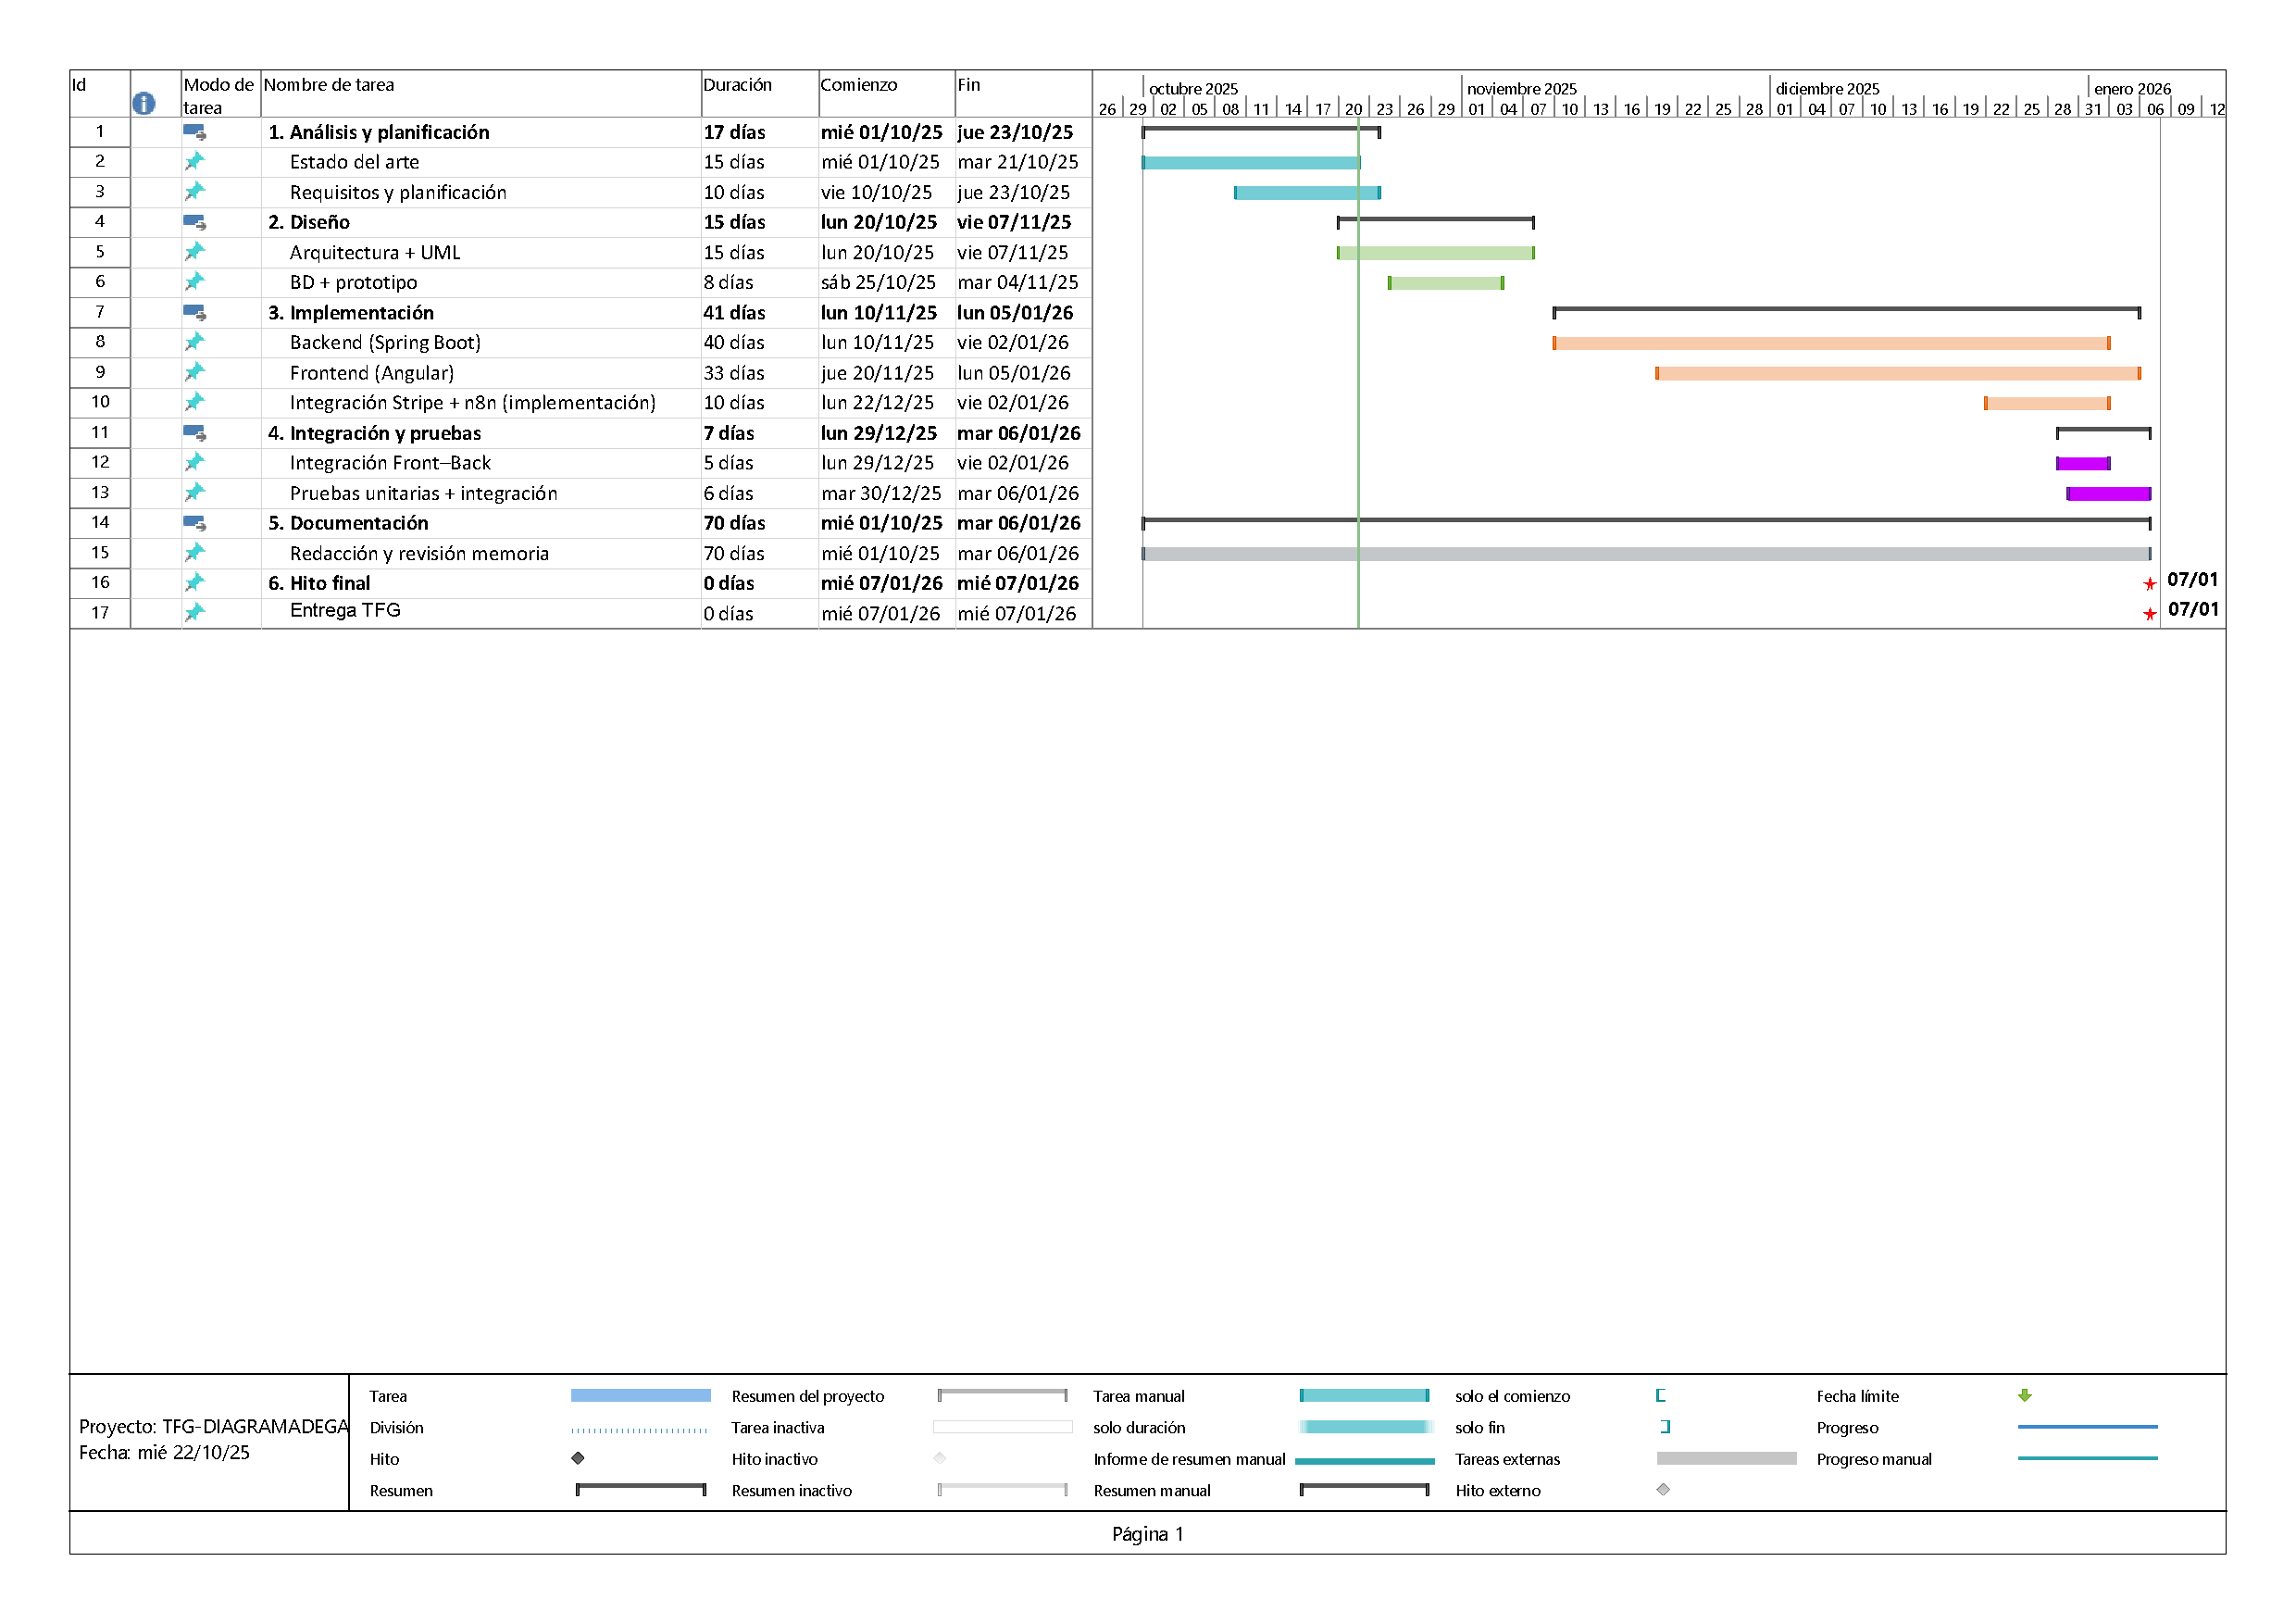
\includegraphics[width=\textwidth]{figs/GanttTodo.pdf}
\caption{Diagrama de Gantt del proyecto (01/10/2025–12/06/2026).}
\end{sidewaysfigure}

\clearpage
\subsection{Estimación de costes}

Para el cálculo de costes se han tenido en cuenta tanto los recursos humanos como los materiales y el software utilizado. 
Aunque el proyecto ha sido desarrollado por una sola persona, se ha desglosado el trabajo según distintos perfiles habituales en el desarrollo de software: 
jefe de proyecto, analista, desarrollador y tester. 
De esta forma se obtiene una estimación más ajustada y realista del esfuerzo requerido.

\begin{table}[H]
\centering
\begin{tabular}{|L{4.5cm}|c|}
\hline
\textbf{Perfil} & \textbf{Horas asignadas} \\
\hline
Jefe de proyecto / Analista & 40 h \\
Desarrollador backend & 140 h \\
Desarrollador frontend & 100 h \\
Tester / Validación & 40 h \\
\hline
\textbf{Total de horas estimadas} & \textbf{320 h} \\
\hline
\end{tabular}
\caption{Reparto de horas por perfil utilizado para la estimación de costes.}
\end{table}

\begin{table}[H]
\centering
\begin{tabular}{|L{4.5cm}|L{7.5cm}|c|}
\hline
\textbf{Concepto} & \textbf{Detalle} & \textbf{Coste estimado} \\
\hline
\textbf{Coste de personal} & Jefe de proyecto / analista: 40 h × 18 €/h & 720 € \\
 & Desarrollador backend: 140 h × 12 €/h & 1.680 € \\
 & Desarrollador frontend: 100 h × 12 €/h & 1.200 € \\
 & Tester / validación: 40 h × 10 €/h & 400 € \\
\hline
\textbf{Subtotal personal} & & \textbf{4.000 €} \\
\hline
\textbf{Seguridad Social (30 \%)} & Aplicado al coste de personal (30 \% × 4.000 €) & \textbf{1.200 €} \\
\hline
\textbf{Coste de software} & Herramientas gratuitas (Angular, Spring Boot, MySQL, VSCode, Postman) & 0 € \\
\hline
\textbf{Coste de software con licencia universitaria} & Visual Paradigm (licencia académica proporcionada por la universidad) & 0 € \\
\hline
\textbf{Coste de hardware (amortizado)} & Portátil personal (1.200 € de valor, amortizado 4 meses sobre 4 años) & 100 € \\
\hline
\textbf{Costes indirectos} & Electricidad, Internet y agua durante el desarrollo (estimado) & 80 € \\
\hline
\textbf{Total estimado del proyecto} & & \textbf{5.380 €} \\
\hline
\end{tabular}
\caption{Estimación de costes detallada por perfil y recursos.}
\vspace{0.3cm}
\textit{Nota: el valor del hardware se ha amortizado en base a una vida útil estimada de cuatro años.}
\end{table}
\clearpage
Además, se incluyen las características del equipo utilizado durante el desarrollo, ya que impactan tanto en la amortización del hardware como en el rendimiento del proceso de trabajo:

\begin{itemize}
    \item \textbf{CPU:} Intel Core i7-12700H
    \item \textbf{RAM:} 16 GB DDR5
    \item \textbf{Almacenamiento:} SSD NVMe 1 TB
    \item \textbf{Gráfica:} NVIDIA RTX 3050 Ti
    \item \textbf{Sistema operativo:} Windows 11
\end{itemize}

Las tarifas horarias aplicadas se han estimado a partir de referencias salariales publicadas en portales de empleo especializados \cite{Indeed2025}.

Finalmente, el coste total del proyecto se obtiene mediante la siguiente expresión:

\[
C_{\text{total}} = C_{\text{personal}} + C_{\text{SeguridadSocial}} + C_{\text{hardware}} + C_{\text{software}} + C_{\text{indirectos}}
\]

\[
C_{\text{total}} = 4\,000 + 1\,200 + 100 + 0 + 80 = \textbf{5\,380\,€}
\]

El resultado confirma que el proyecto mantiene un coste razonable y acorde a su nivel de complejidad. 
El uso de herramientas libres y de una infraestructura propia reduce significativamente el coste total, 
manteniendo una buena relación entre esfuerzo, recursos y resultados obtenidos.


% Riesgos que pueden incurrir en el desarrollo del sistema
\clearpage
\section{Riesgos}

La gestión de riesgos permite anticipar posibles incidencias y definir estrategias preventivas que minimicen su impacto en el desarrollo del proyecto. 
En la siguiente tabla se resumen los principales riesgos identificados junto con su probabilidad, impacto y categoría general.

\begin{table}[H]
\centering
\begin{tabular}{|L{6.5cm}|c|c|c|}
\hline
\textbf{Riesgo identificado} & \textbf{Probabilidad} & \textbf{Impacto} & \textbf{Categoría} \\
\hline
Problemas de integración entre módulos Angular–Spring Boot & Media & Alta & Técnica \\
\hline
Fallos en la pasarela de pago (Stripe) & Baja & Alta & Técnica \\
\hline
Cambios en los requisitos durante el desarrollo & Media & Media & Gestión \\
\hline
Sobrecarga de trabajo o retrasos en la planificación & Media & Media & Organización \\
\hline
Fallos de seguridad en la API o la base de datos & Baja & Alta & Seguridad \\
\hline
Falta de experiencia inicial con el bot de Telegram & Media & Media & Técnica \\
\hline
\end{tabular}
\caption{Principales riesgos identificados durante el desarrollo del proyecto.}
\end{table}

A continuación, se describen las medidas generales de \textbf{mitigación y contingencia} aplicadas a los riesgos identificados:

\begin{itemize}
    \item \textbf{Problemas de integración entre módulos Angular–Spring Boot:} se establecerán pruebas de integración progresivas conforme se incorporen nuevos módulos al sistema, garantizando la detección temprana de errores. Asimismo, se mantendrá una estructura de código modular que facilite la interoperabilidad entre el frontend y el backend.

    \item \textbf{Fallos en la pasarela de pago (Stripe):} con anterioridad a la activación de los pagos reales, se realizarán pruebas exhaustivas en el entorno de simulación que proporciona la plataforma. Ante un eventual fallo, el sistema contempla la posibilidad de reintentar el pago o registrar el pedido pendiente para su revisión posterior.

    \item \textbf{Cambios en los requisitos durante el desarrollo:} se reservará un margen de tiempo en la planificación que permita absorber cambios de alcance sin comprometer las funcionalidades principales. Asimismo, se mantendrá en todo momento una versión operativa del sistema, priorizando los requisitos de mayor relevancia.

    \item \textbf{Sobrecarga de trabajo o retrasos en la planificación:} el trabajo se organizará en tareas de alcance reducido con objetivos semanales verificables. Adicionalmente, se incorporará un margen de contingencia en la planificación para absorber posibles imprevistos o revisiones no previstas inicialmente.

    \item \textbf{Fallos de seguridad en la aplicación o base de datos:} se realizarán copias de seguridad periódicas y se aplicarán mecanismos de almacenamiento seguro de credenciales. Asimismo, se mantendrán actualizadas las dependencias y herramientas del proyecto para minimizar la exposición a vulnerabilidades conocidas.

    \item \textbf{Falta de experiencia con el bot de Telegram:} se destinará un periodo de aprendizaje previo a la integración completa, durante el cual se desarrollarán prototipos sencillos para comprender la gestión de comandos y notificaciones. La documentación oficial de la librería servirá como referencia principal durante todo el proceso.
\end{itemize}
Gracias a estas medidas, se espera que los riesgos identificados tengan un impacto limitado en el desarrollo y no comprometan los objetivos principales del proyecto.



% Viabilidad del proyecto presentado
\section{Viabilidad}

\subsection{Viabilidad legal}

El proyecto no presenta impedimentos legales, ya que no maneja datos personales sensibles y cumple con la normativa vigente, especialmente con el Reglamento General de Protección de Datos (RGPD). 
Los pagos se realizan mediante la plataforma \textbf{Stripe}, que se encarga de procesar la información de forma segura y cifrada, evitando que el sistema tenga que almacenar datos de tarjetas. 
Todas las tecnologías empleadas son de \textbf{código abierto} o disponen de \textbf{licencias académicas gratuitas}, por lo que su uso es totalmente legal en el contexto de un proyecto universitario.

\subsection{Viabilidad técnica}

El uso conjunto de \textbf{Angular}, \textbf{Spring Boot}, \textbf{MySQL} y el \textbf{bot de Telegram} proporciona una solución estable, escalable y fácil de mantener.
Son herramientas actuales, bien documentadas y con una amplia comunidad de desarrolladores, lo que facilita la resolución de problemas y reduce el riesgo de incompatibilidades.
Además, el diseño modular del sistema permite incorporar futuras mejoras, como nuevos métodos de pago o notificaciones adicionales, sin necesidad de modificar la estructura principal del proyecto.

\subsection{Viabilidad económica}

El proyecto resulta \textbf{económicamente viable}, ya que su desarrollo no requiere inversión en licencias ni en infraestructura adicional. 
El software utilizado es \textbf{gratuito y de código abierto}, y el equipo empleado para el desarrollo es personal, por lo que los únicos costes reales corresponden al tiempo de dedicación y al uso del propio ordenador. 
Teniendo en cuenta que el coste total estimado del proyecto es de aproximadamente \textbf{5.380 €}, se puede concluir que se trata de una solución accesible, eficiente y sostenible para un entorno académico o de pequeña empresa.


\chapter{Análisis}
% Contenidos del capítulo.
% Las secciones presentadas son orientativas y no representan
% necesariamente la organización que debe tener este capítulo.

\section{Diagramas de análisis}

\subsection{Diagrama de casos de uso}

Para representar las interacciones entre los diferentes actores del sistema se ha elaborado el diagrama de casos de uso mostrado en la Figura~\ref{fig:casos_uso}. 
Este permite visualizar de forma general las funcionalidades principales y la relación entre el cliente, el administrador y el \textit{bot de Telegram}.

\begin{figure}[H]
    \centering
    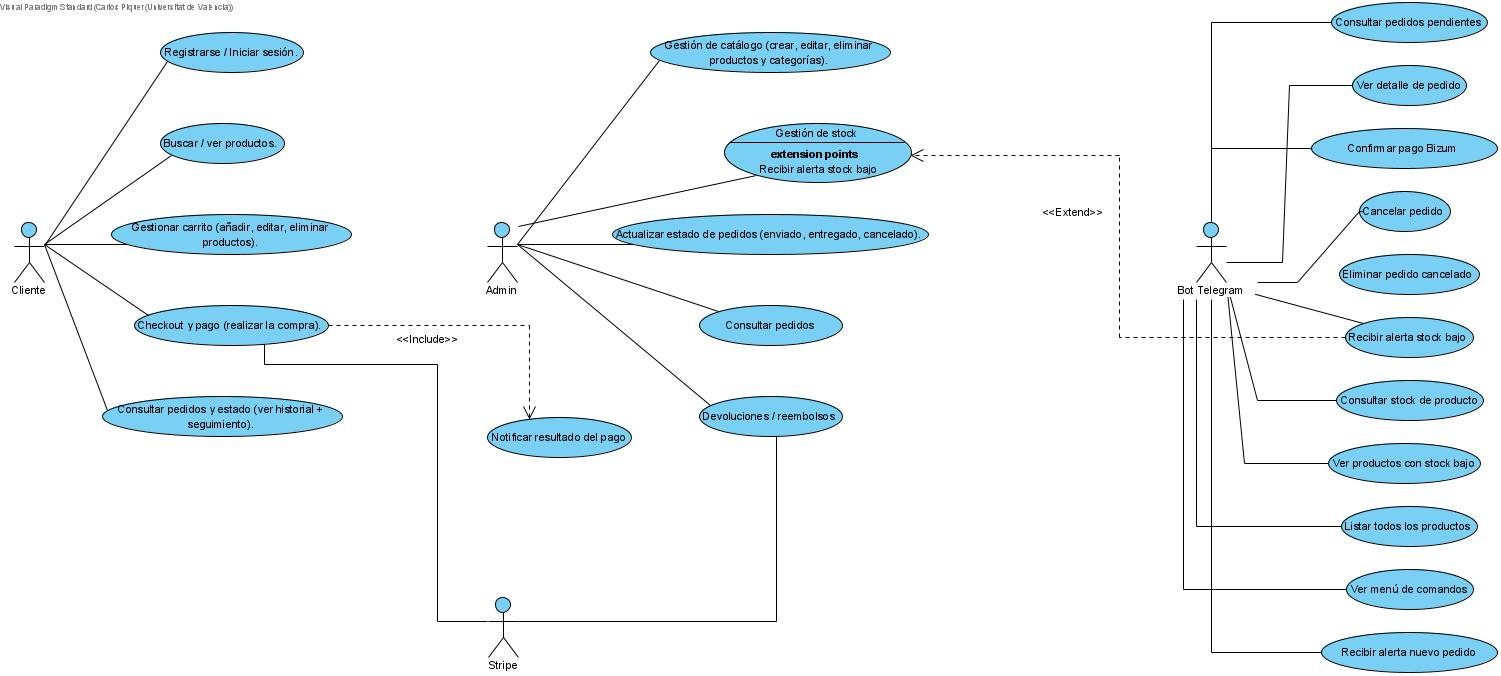
\includegraphics[height=1\textwidth, width=1.05\textwidth, keepaspectratio]{figs/casos_de_uso_goodv2.jpg}
    \caption{Diagrama de casos de uso del sistema.}
    \label{fig:casos_uso}
\end{figure}
\clearpage

\subsection{Especificación de casos de uso}

A continuación se especifica, en formato tabular, el detalle de cada uno de los casos de uso identificados en el diagrama anterior. Los casos de uso se agrupan por actor: cliente, administrador, Stripe y bot de Telegram.

\subsubsection{CU-01 Registrarse / iniciar sesión}

\begin{table}[H]
\centering
\small
\begin{tabular}{|m{0.28\textwidth}|m{0.65\textwidth}|}
\hline
\textbf{Nombre} & CU-01 Registrarse / iniciar sesión \\ \hline
\textbf{Actor(es)} & Cliente \\ \hline
\textbf{Descripción} & El cliente puede registrarse como nuevo usuario o iniciar sesión con sus credenciales. \\ \hline
\textbf{Precondiciones} & El sistema debe estar accesible. Para iniciar sesión, el usuario debe estar registrado previamente. \\ \hline
\textbf{Postcondiciones} & El cliente queda autenticado y accede a las funcionalidades reservadas para usuarios registrados. \\ \hline
\textbf{Flujo principal} & 1. El cliente accede a la pantalla de registro o inicio de sesión. \newline 2. Introduce sus datos (correo electrónico y contraseña). \newline 3. El sistema valida las credenciales. \newline 4. El cliente queda autenticado y es redirigido al inicio. \\ \hline
\textbf{Flujos alternativos} & 3.a Credenciales incorrectas $\rightarrow$ el sistema muestra un mensaje de error. \newline 3.b Correo ya registrado (en registro) $\rightarrow$ el sistema informa del duplicado. \\ \hline
\textbf{Requisitos funcionales relacionados} & RF-01 \\ \hline
\end{tabular}
\caption{Especificación del caso de uso CU-01 — Registrarse / iniciar sesión.}
\end{table}

\subsubsection{CU-02 Buscar / ver productos}

\begin{table}[H]
\centering
\small
\begin{tabular}{|m{0.28\textwidth}|m{0.65\textwidth}|}
\hline
\textbf{Nombre} & CU-02 Buscar / ver productos \\ \hline
\textbf{Actor(es)} & Cliente \\ \hline
\textbf{Descripción} & El cliente explora el catálogo, aplica filtros por categoría y precio, y realiza búsquedas por nombre de producto. \\ \hline
\textbf{Precondiciones} & El catálogo debe contener productos disponibles. \\ \hline
\textbf{Postcondiciones} & El cliente visualiza los productos que cumplen los criterios de búsqueda o filtrado. \\ \hline
\textbf{Flujo principal} & 1. El cliente accede a la sección de catálogo. \newline 2. Aplica filtros opcionales o introduce un término de búsqueda. \newline 3. El sistema devuelve y muestra los resultados correspondientes. \\ \hline
\textbf{Flujos alternativos} & 3.a Ningún producto coincide con los criterios $\rightarrow$ el sistema muestra un mensaje informativo. \\ \hline
\textbf{Requisitos funcionales relacionados} & RF-02 \\ \hline
\end{tabular}
\caption{Especificación del caso de uso CU-02 — Buscar / ver productos.}
\end{table}

\subsubsection{CU-03 Gestionar carrito}

\begin{table}[H]
\centering
\small
\begin{tabular}{|m{0.28\textwidth}|m{0.65\textwidth}|}
\hline
\textbf{Nombre} & CU-03 Gestionar carrito \\ \hline
\textbf{Actor(es)} & Cliente \\ \hline
\textbf{Descripción} & El cliente añade productos al carrito, modifica cantidades o elimina artículos. \\ \hline
\textbf{Precondiciones} & El cliente debe estar autenticado y el catálogo debe estar operativo. \\ \hline
\textbf{Postcondiciones} & El carrito queda actualizado con los productos y cantidades seleccionados. \\ \hline
\textbf{Flujo principal} & 1. El cliente selecciona un producto del catálogo. \newline 2. Lo añade al carrito. \newline 3. La WebApp actualiza las unidades y el total del carrito. \newline 4. El cliente puede modificar cantidades o eliminar artículos. \newline 5. El sistema mantiene los datos sincronizados. \\ \hline
\textbf{Flujos alternativos} & 2.a Stock insuficiente $\rightarrow$ el sistema muestra un aviso. \newline 1.a El cliente no dispone de carrito activo $\rightarrow$ el sistema crea uno automáticamente. \\ \hline
\textbf{Requisitos funcionales relacionados} & RF-03 \\ \hline
\end{tabular}
\caption{Especificación del caso de uso CU-03 — Gestionar carrito.}
\end{table}

\clearpage

\subsubsection{CU-04 Checkout y pago}

\begin{table}[H]
\centering
\small
\begin{tabular}{|m{0.28\textwidth}|m{0.65\textwidth}|}
\hline
\textbf{Nombre} & CU-04 Checkout y pago \\ \hline
\textbf{Actor(es)} & Cliente, Stripe \\ \hline
\textbf{Descripción} & El cliente completa el proceso de compra introduciendo sus datos personales y de pago. El pago es procesado por la pasarela Stripe. Incluye CU-11 (\textit{Notificar resultado del pago}). \\ \hline
\textbf{Precondiciones} & El cliente debe estar autenticado y disponer de un carrito con productos. \\ \hline
\textbf{Postcondiciones} & El pedido queda registrado como pagado y se genera la factura correspondiente. \\ \hline
\textbf{Flujo principal} & 1. El cliente accede al checkout. \newline 2. Introduce sus datos personales y dirección de envío. \newline 3. Selecciona el método de pago. \newline 4. La WebApp crea el pedido en estado ``pendiente''. \newline 5. Stripe procesa el pago. \newline 6. Stripe notifica el resultado (CU-11). \newline 7. La WebApp confirma el pedido y genera la factura. \\ \hline
\textbf{Flujos alternativos} & 5.a Stripe requiere autenticación adicional (3D Secure). \newline 5.b Pago rechazado $\rightarrow$ el sistema muestra un mensaje de error y el pedido no se completa. \\ \hline
\textbf{Requisitos funcionales relacionados} & RF-04, RF-06 \\ \hline
\end{tabular}
\caption{Especificación del caso de uso CU-04 — Checkout y pago.}
\end{table}

\subsubsection{CU-05 Consultar pedidos y estado}

\begin{table}[H]
\centering
\small
\begin{tabular}{|m{0.28\textwidth}|m{0.65\textwidth}|}
\hline
\textbf{Nombre} & CU-05 Consultar pedidos y estado \\ \hline
\textbf{Actor(es)} & Cliente \\ \hline
\textbf{Descripción} & El cliente consulta el historial de sus pedidos anteriores y el estado actualizado de cada uno. \\ \hline
\textbf{Precondiciones} & El cliente debe estar autenticado y haber realizado al menos un pedido. \\ \hline
\textbf{Postcondiciones} & El cliente visualiza el historial de pedidos con sus estados actualizados. \\ \hline
\textbf{Flujo principal} & 1. El cliente accede a su área personal. \newline 2. Selecciona la sección de historial de pedidos. \newline 3. El sistema muestra el listado de pedidos con su estado y detalle. \\ \hline
\textbf{Flujos alternativos} & 3.a No existen pedidos $\rightarrow$ el sistema muestra un mensaje informativo. \\ \hline
\textbf{Requisitos funcionales relacionados} & RF-08 \\ \hline
\end{tabular}
\caption{Especificación del caso de uso CU-05 — Consultar pedidos y estado.}
\end{table}

\clearpage

\subsubsection{CU-06 Gestión de catálogo}

\begin{table}[H]
\centering
\small
\begin{tabular}{|m{0.28\textwidth}|m{0.65\textwidth}|}
\hline
\textbf{Nombre} & CU-06 Gestión de catálogo \\ \hline
\textbf{Actor(es)} & Administrador \\ \hline
\textbf{Descripción} & El administrador crea, edita y elimina productos y categorías del catálogo de la tienda. \\ \hline
\textbf{Precondiciones} & El administrador debe estar autenticado con permisos de administración. \\ \hline
\textbf{Postcondiciones} & Los cambios en el catálogo quedan reflejados de forma inmediata en la tienda. \\ \hline
\textbf{Flujo principal} & 1. El administrador accede al panel de administración. \newline 2. Selecciona la sección de catálogo. \newline 3. Crea, edita o elimina un producto o categoría. \newline 4. El sistema actualiza el catálogo. \\ \hline
\textbf{Flujos alternativos} & 3.a Datos del producto incompletos $\rightarrow$ el sistema solicita corrección. \newline 3.b Eliminación de producto con pedidos activos $\rightarrow$ el sistema muestra un aviso. \\ \hline
\textbf{Requisitos funcionales relacionados} & RF-05 \\ \hline
\end{tabular}
\caption{Especificación del caso de uso CU-06 — Gestión de catálogo.}
\end{table}

\subsubsection{CU-07 Gestión de stock}

\begin{table}[H]
\centering
\small
\begin{tabular}{|m{0.28\textwidth}|m{0.65\textwidth}|}
\hline
\textbf{Nombre} & CU-07 Gestión de stock \\ \hline
\textbf{Actor(es)} & Administrador \\ \hline
\textbf{Descripción} & El administrador actualiza manualmente el stock de los productos. Si el valor resultante es inferior al umbral configurado, se extiende el caso de uso con el envío automático de una alerta (CU-18). \\ \hline
\textbf{Precondiciones} & El administrador debe estar autenticado. \\ \hline
\textbf{Postcondiciones} & El stock del producto queda actualizado. Si el nuevo valor está por debajo del umbral, se genera una alerta automática. \\ \hline
\textbf{Flujo principal} & 1. El administrador accede al panel de administración. \newline 2. Selecciona un producto y modifica su valor de stock. \newline 3. El sistema guarda el nuevo valor. \\ \hline
\textbf{Flujos alternativos} & 3.a El nuevo stock es inferior al umbral $\rightarrow$ el sistema extiende con CU-18 (alerta de bajo stock). \\ \hline
\textbf{Requisitos funcionales relacionados} & RF-05, RF-07 \\ \hline
\end{tabular}
\caption{Especificación del caso de uso CU-07 — Gestión de stock.}
\end{table}

\subsubsection{CU-08 Actualizar estado de pedidos}

\begin{table}[H]
\centering
\small
\begin{tabular}{|m{0.28\textwidth}|m{0.65\textwidth}|}
\hline
\textbf{Nombre} & CU-08 Actualizar estado de pedidos \\ \hline
\textbf{Actor(es)} & Administrador \\ \hline
\textbf{Descripción} & El administrador actualiza el estado de los pedidos recibidos: enviado, entregado o cancelado. \\ \hline
\textbf{Precondiciones} & El administrador debe estar autenticado y deben existir pedidos en el sistema. \\ \hline
\textbf{Postcondiciones} & El estado del pedido queda actualizado en el sistema. \\ \hline
\textbf{Flujo principal} & 1. El administrador accede a la sección de pedidos. \newline 2. Selecciona un pedido concreto. \newline 3. Cambia el estado al valor correspondiente. \newline 4. El sistema guarda el nuevo estado. \\ \hline
\textbf{Flujos alternativos} & — No aplica. \\ \hline
\textbf{Requisitos funcionales relacionados} & RF-08 \\ \hline
\end{tabular}
\caption{Especificación del caso de uso CU-08 — Actualizar estado de pedidos.}
\end{table}

\clearpage

\subsubsection{CU-09 Consultar pedidos}

\begin{table}[H]
\centering
\small
\begin{tabular}{|m{0.28\textwidth}|m{0.65\textwidth}|}
\hline
\textbf{Nombre} & CU-09 Consultar pedidos \\ \hline
\textbf{Actor(es)} & Administrador \\ \hline
\textbf{Descripción} & El administrador consulta el listado completo de pedidos del sistema, con la posibilidad de filtrar por estado. \\ \hline
\textbf{Precondiciones} & El administrador debe estar autenticado. \\ \hline
\textbf{Postcondiciones} & El administrador visualiza el listado de pedidos con la información relevante. \\ \hline
\textbf{Flujo principal} & 1. El administrador accede a la sección de pedidos. \newline 2. Aplica filtros opcionales por estado. \newline 3. El sistema muestra el listado de pedidos. \\ \hline
\textbf{Flujos alternativos} & 3.a No hay pedidos $\rightarrow$ el sistema muestra un mensaje informativo. \\ \hline
\textbf{Requisitos funcionales relacionados} & RF-08 \\ \hline
\end{tabular}
\caption{Especificación del caso de uso CU-09 — Consultar pedidos.}
\end{table}

\subsubsection{CU-10 Devoluciones / reembolsos}

\begin{table}[H]
\centering
\small
\begin{tabular}{|m{0.28\textwidth}|m{0.65\textwidth}|}
\hline
\textbf{Nombre} & CU-10 Devoluciones / reembolsos \\ \hline
\textbf{Actor(es)} & Administrador \\ \hline
\textbf{Descripción} & El administrador gestiona las solicitudes de devolución o reembolso de pedidos. \\ \hline
\textbf{Precondiciones} & El administrador debe estar autenticado y debe existir un pedido susceptible de devolución. \\ \hline
\textbf{Postcondiciones} & El pedido queda marcado como devuelto o reembolsado y el stock se repone si procede. \\ \hline
\textbf{Flujo principal} & 1. El administrador accede al detalle de un pedido. \newline 2. Selecciona la opción de devolución o reembolso. \newline 3. El sistema actualiza el estado del pedido. \newline 4. Si procede, el stock de los artículos devueltos se restaura. \\ \hline
\textbf{Flujos alternativos} & 3.a El pedido no es elegible para devolución $\rightarrow$ el sistema muestra un aviso. \\ \hline
\textbf{Requisitos funcionales relacionados} & RF-08 \\ \hline
\end{tabular}
\caption{Especificación del caso de uso CU-10 — Devoluciones / reembolsos.}
\end{table}

\subsubsection{CU-11 Notificar resultado del pago}

\begin{table}[H]
\centering
\small
\begin{tabular}{|m{0.28\textwidth}|m{0.65\textwidth}|}
\hline
\textbf{Nombre} & CU-11 Notificar resultado del pago \\ \hline
\textbf{Actor(es)} & Stripe \\ \hline
\textbf{Descripción} & Stripe notifica a la WebApp el resultado del procesamiento del pago (confirmación o rechazo). Este caso de uso es incluido por CU-04 (\textit{Checkout y pago}). \\ \hline
\textbf{Precondiciones} & El cliente debe haber iniciado el proceso de pago en el checkout. \\ \hline
\textbf{Postcondiciones} & La WebApp recibe y procesa el resultado, actualizando el estado del pedido. \\ \hline
\textbf{Flujo principal} & 1. Stripe procesa la transacción. \newline 2. Stripe envía la notificación del resultado a la WebApp. \newline 3. La WebApp actualiza el estado del pedido en consecuencia. \\ \hline
\textbf{Flujos alternativos} & 2.a Error de comunicación $\rightarrow$ la WebApp reintenta la confirmación. \\ \hline
\textbf{Requisitos funcionales relacionados} & RF-04 \\ \hline
\end{tabular}
\caption{Especificación del caso de uso CU-11 — Notificar resultado del pago.}
\end{table}

\clearpage

\subsubsection{CU-12 Recibir alerta nuevo pedido}

\begin{table}[H]
\centering
\small
\begin{tabular}{|m{0.28\textwidth}|m{0.65\textwidth}|}
\hline
\textbf{Nombre} & CU-12 Recibir alerta nuevo pedido \\ \hline
\textbf{Actor(es)} & Bot de Telegram \\ \hline
\textbf{Descripción} & El bot de Telegram recibe una notificación automática cada vez que se confirma un nuevo pedido y la transmite al administrador. \\ \hline
\textbf{Precondiciones} & El bot de Telegram debe estar activo y el pedido debe estar confirmado. \\ \hline
\textbf{Postcondiciones} & El administrador recibe la notificación de nuevo pedido en Telegram. \\ \hline
\textbf{Flujo principal} & 1. La WebApp detecta un nuevo pedido confirmado. \newline 2. Notifica al bot de Telegram. \newline 3. El bot envía un mensaje de aviso al administrador. \\ \hline
\textbf{Flujos alternativos} & 3.a Error de envío $\rightarrow$ el bot registra el error e intenta reenviar. \\ \hline
\textbf{Requisitos funcionales relacionados} & RF-07 \\ \hline
\end{tabular}
\caption{Especificación del caso de uso CU-12 — Recibir alerta nuevo pedido.}
\end{table}

\subsubsection{CU-13 Consultar pedidos pendientes}

\begin{table}[H]
\centering
\small
\begin{tabular}{|m{0.28\textwidth}|m{0.65\textwidth}|}
\hline
\textbf{Nombre} & CU-13 Consultar pedidos pendientes \\ \hline
\textbf{Actor(es)} & Bot de Telegram \\ \hline
\textbf{Descripción} & Mediante un comando de Telegram, el administrador solicita al bot el listado de pedidos pendientes de procesamiento. \\ \hline
\textbf{Precondiciones} & El bot de Telegram debe estar activo. \\ \hline
\textbf{Postcondiciones} & El administrador recibe el listado de pedidos pendientes en Telegram. \\ \hline
\textbf{Flujo principal} & 1. El administrador envía el comando correspondiente al bot. \newline 2. El bot consulta los pedidos en estado ``pendiente''. \newline 3. El bot devuelve el listado al administrador. \\ \hline
\textbf{Flujos alternativos} & 3.a No hay pedidos pendientes $\rightarrow$ el bot responde con un mensaje informativo. \\ \hline
\textbf{Requisitos funcionales relacionados} & RF-07, RF-08 \\ \hline
\end{tabular}
\caption{Especificación del caso de uso CU-13 — Consultar pedidos pendientes.}
\end{table}

\subsubsection{CU-14 Ver detalle de pedido}

\begin{table}[H]
\centering
\small
\begin{tabular}{|m{0.28\textwidth}|m{0.65\textwidth}|}
\hline
\textbf{Nombre} & CU-14 Ver detalle de pedido \\ \hline
\textbf{Actor(es)} & Bot de Telegram \\ \hline
\textbf{Descripción} & El administrador solicita al bot el detalle completo de un pedido concreto mediante su identificador. \\ \hline
\textbf{Precondiciones} & El bot de Telegram debe estar activo y el pedido debe existir en el sistema. \\ \hline
\textbf{Postcondiciones} & El administrador recibe los datos del pedido por Telegram. \\ \hline
\textbf{Flujo principal} & 1. El administrador envía el identificador del pedido al bot. \newline 2. El bot consulta los detalles en el sistema. \newline 3. El bot devuelve la información completa del pedido. \\ \hline
\textbf{Flujos alternativos} & 3.a El pedido no existe $\rightarrow$ el bot indica que no se ha encontrado. \\ \hline
\textbf{Requisitos funcionales relacionados} & RF-08 \\ \hline
\end{tabular}
\caption{Especificación del caso de uso CU-14 — Ver detalle de pedido.}
\end{table}

\clearpage

\subsubsection{CU-15 Confirmar pago Bizum}

\begin{table}[H]
\centering
\small
\begin{tabular}{|m{0.28\textwidth}|m{0.65\textwidth}|}
\hline
\textbf{Nombre} & CU-15 Confirmar pago Bizum \\ \hline
\textbf{Actor(es)} & Bot de Telegram \\ \hline
\textbf{Descripción} & El administrador confirma manualmente a través del bot que ha recibido el pago por Bizum de un pedido pendiente. \\ \hline
\textbf{Precondiciones} & Debe existir un pedido en estado ``pendiente de pago'' por Bizum. \\ \hline
\textbf{Postcondiciones} & El pedido queda marcado como pagado en el sistema. \\ \hline
\textbf{Flujo principal} & 1. El administrador envía el comando de confirmación de Bizum con el identificador del pedido. \newline 2. El bot actualiza el estado del pedido a ``pagado''. \newline 3. El bot confirma la acción al administrador. \\ \hline
\textbf{Flujos alternativos} & 2.a El pedido no se encuentra o ya está pagado $\rightarrow$ el bot informa del error. \\ \hline
\textbf{Requisitos funcionales relacionados} & RF-04 \\ \hline
\end{tabular}
\caption{Especificación del caso de uso CU-15 — Confirmar pago Bizum.}
\end{table}

\subsubsection{CU-16 Cancelar pedido}

\begin{table}[H]
\centering
\small
\begin{tabular}{|m{0.28\textwidth}|m{0.65\textwidth}|}
\hline
\textbf{Nombre} & CU-16 Cancelar pedido \\ \hline
\textbf{Actor(es)} & Bot de Telegram \\ \hline
\textbf{Descripción} & El administrador cancela un pedido activo a través de un comando del bot de Telegram. \\ \hline
\textbf{Precondiciones} & El bot de Telegram debe estar activo y el pedido debe encontrarse en un estado cancelable. \\ \hline
\textbf{Postcondiciones} & El pedido queda marcado como cancelado y el stock asociado se libera. \\ \hline
\textbf{Flujo principal} & 1. El administrador envía el comando de cancelación con el identificador del pedido. \newline 2. El bot actualiza el estado del pedido a ``cancelado''. \newline 3. El bot libera el stock asociado y confirma la cancelación. \\ \hline
\textbf{Flujos alternativos} & 2.a El pedido ya fue entregado $\rightarrow$ el bot informa de que no es posible cancelarlo. \\ \hline
\textbf{Requisitos funcionales relacionados} & RF-08 \\ \hline
\end{tabular}
\caption{Especificación del caso de uso CU-16 — Cancelar pedido.}
\end{table}

\subsubsection{CU-17 Eliminar pedido cancelado}

\begin{table}[H]
\centering
\small
\begin{tabular}{|m{0.28\textwidth}|m{0.65\textwidth}|}
\hline
\textbf{Nombre} & CU-17 Eliminar pedido cancelado \\ \hline
\textbf{Actor(es)} & Bot de Telegram \\ \hline
\textbf{Descripción} & El administrador solicita al bot la eliminación definitiva de un pedido previamente cancelado. \\ \hline
\textbf{Precondiciones} & El pedido debe encontrarse en estado ``cancelado''. \\ \hline
\textbf{Postcondiciones} & El pedido queda eliminado del sistema de forma permanente. \\ \hline
\textbf{Flujo principal} & 1. El administrador envía el comando de eliminación con el identificador del pedido. \newline 2. El bot verifica que el pedido está en estado cancelado. \newline 3. El bot elimina el pedido del sistema y confirma la acción. \\ \hline
\textbf{Flujos alternativos} & 2.a El pedido no está cancelado $\rightarrow$ el bot informa de que no es posible eliminarlo. \\ \hline
\textbf{Requisitos funcionales relacionados} & RF-08 \\ \hline
\end{tabular}
\caption{Especificación del caso de uso CU-17 — Eliminar pedido cancelado.}
\end{table}

\clearpage

\subsubsection{CU-18 Recibir alerta de stock bajo}

\begin{table}[H]
\centering
\small
\begin{tabular}{|m{0.28\textwidth}|m{0.65\textwidth}|}
\hline
\textbf{Nombre} & CU-18 Recibir alerta de stock bajo \\ \hline
\textbf{Actor(es)} & Bot de Telegram \\ \hline
\textbf{Descripción} & Cuando el stock de un producto cae por debajo del umbral configurado, el bot envía automáticamente una alerta al administrador. Este caso de uso extiende a CU-07 (\textit{Gestión de stock}). \\ \hline
\textbf{Precondiciones} & Debe existir al menos un producto con stock inferior al umbral mínimo configurado. \\ \hline
\textbf{Postcondiciones} & El administrador recibe una alerta de bajo stock en Telegram. \\ \hline
\textbf{Flujo principal} & 1. La WebApp detecta que el stock de un producto ha descendido por debajo del umbral. \newline 2. Notifica al bot de Telegram. \newline 3. El bot envía una alerta al administrador indicando el producto afectado y el stock restante. \\ \hline
\textbf{Flujos alternativos} & — No aplica. \\ \hline
\textbf{Requisitos funcionales relacionados} & RF-07 \\ \hline
\end{tabular}
\caption{Especificación del caso de uso CU-18 — Recibir alerta de stock bajo.}
\end{table}

\subsubsection{CU-19 Consultar stock de producto}

\begin{table}[H]
\centering
\small
\begin{tabular}{|m{0.28\textwidth}|m{0.65\textwidth}|}
\hline
\textbf{Nombre} & CU-19 Consultar stock de producto \\ \hline
\textbf{Actor(es)} & Bot de Telegram \\ \hline
\textbf{Descripción} & El administrador consulta el stock actual de un producto concreto a través de un comando del bot. \\ \hline
\textbf{Precondiciones} & El bot de Telegram debe estar activo. \\ \hline
\textbf{Postcondiciones} & El administrador recibe el nivel de stock actual del producto solicitado. \\ \hline
\textbf{Flujo principal} & 1. El administrador envía el comando de consulta con el nombre o identificador del producto. \newline 2. El bot consulta el stock en el sistema. \newline 3. El bot responde con el valor de stock actual. \\ \hline
\textbf{Flujos alternativos} & 3.a El producto no existe $\rightarrow$ el bot informa de que no se ha encontrado. \\ \hline
\textbf{Requisitos funcionales relacionados} & RF-05 \\ \hline
\end{tabular}
\caption{Especificación del caso de uso CU-19 — Consultar stock de producto.}
\end{table}

\subsubsection{CU-20 Ver productos con stock bajo}

\begin{table}[H]
\centering
\small
\begin{tabular}{|m{0.28\textwidth}|m{0.65\textwidth}|}
\hline
\textbf{Nombre} & CU-20 Ver productos con stock bajo \\ \hline
\textbf{Actor(es)} & Bot de Telegram \\ \hline
\textbf{Descripción} & El administrador solicita al bot el listado de productos cuyo stock se encuentra por debajo del umbral configurado. \\ \hline
\textbf{Precondiciones} & El bot de Telegram debe estar activo. \\ \hline
\textbf{Postcondiciones} & El administrador recibe el listado de productos con stock crítico. \\ \hline
\textbf{Flujo principal} & 1. El administrador envía el comando correspondiente. \newline 2. El bot consulta los productos con stock bajo. \newline 3. El bot responde con el listado de productos y sus niveles de stock. \\ \hline
\textbf{Flujos alternativos} & 3.a No hay productos con stock bajo $\rightarrow$ el bot responde con un mensaje informativo. \\ \hline
\textbf{Requisitos funcionales relacionados} & RF-07 \\ \hline
\end{tabular}
\caption{Especificación del caso de uso CU-20 — Ver productos con stock bajo.}
\end{table}

\clearpage

\subsubsection{CU-21 Listar todos los productos}

\begin{table}[H]
\centering
\small
\begin{tabular}{|m{0.28\textwidth}|m{0.65\textwidth}|}
\hline
\textbf{Nombre} & CU-21 Listar todos los productos \\ \hline
\textbf{Actor(es)} & Bot de Telegram \\ \hline
\textbf{Descripción} & El administrador solicita al bot el listado completo de productos disponibles en el sistema. \\ \hline
\textbf{Precondiciones} & El bot de Telegram debe estar activo y existir productos en el catálogo. \\ \hline
\textbf{Postcondiciones} & El administrador recibe el listado de todos los productos. \\ \hline
\textbf{Flujo principal} & 1. El administrador envía el comando de listado. \newline 2. El bot consulta todos los productos del sistema. \newline 3. El bot responde con el listado completo. \\ \hline
\textbf{Flujos alternativos} & 3.a No hay productos en el catálogo $\rightarrow$ el bot responde con un mensaje informativo. \\ \hline
\textbf{Requisitos funcionales relacionados} & RF-02 \\ \hline
\end{tabular}
\caption{Especificación del caso de uso CU-21 — Listar todos los productos.}
\end{table}

\subsubsection{CU-22 Ver menú de comandos}

\begin{table}[H]
\centering
\small
\begin{tabular}{|m{0.28\textwidth}|m{0.65\textwidth}|}
\hline
\textbf{Nombre} & CU-22 Ver menú de comandos \\ \hline
\textbf{Actor(es)} & Bot de Telegram \\ \hline
\textbf{Descripción} & El administrador solicita al bot el menú de comandos disponibles para conocer las funcionalidades accesibles. \\ \hline
\textbf{Precondiciones} & El bot de Telegram debe estar activo. \\ \hline
\textbf{Postcondiciones} & El administrador recibe el listado de comandos disponibles con su descripción. \\ \hline
\textbf{Flujo principal} & 1. El administrador envía el comando \texttt{/help} o \texttt{/menu} al bot. \newline 2. El bot responde con el listado completo de comandos disponibles y su descripción. \\ \hline
\textbf{Flujos alternativos} & — No aplica. \\ \hline
\textbf{Requisitos funcionales relacionados} & RF-07 \\ \hline
\end{tabular}
\caption{Especificación del caso de uso CU-22 — Ver menú de comandos.}
\end{table}

\clearpage

\subsection{Diagrama de clases de análisis}

En la Figura~\ref{fig:clases_analisis} se muestra el \textbf{diagrama de clases de análisis} del sistema. 
Este modelo conceptual identifica las principales entidades que intervienen en el dominio de la aplicación, 
así como las relaciones que existen entre ellas. 
El cliente dispone de un carrito y puede realizar múltiples pedidos, 
cada uno de los cuales está asociado a un pago y a varios productos. 
Además, el cliente puede almacenar varias direcciones de envío, 
y los productos se agrupan dentro de categorías. 
El diagrama abstrae los detalles técnicos y se centra únicamente en los conceptos del negocio, 
sirviendo como base para el posterior diagrama de clases de diseño.

\begin{figure}[H]
    \centering
    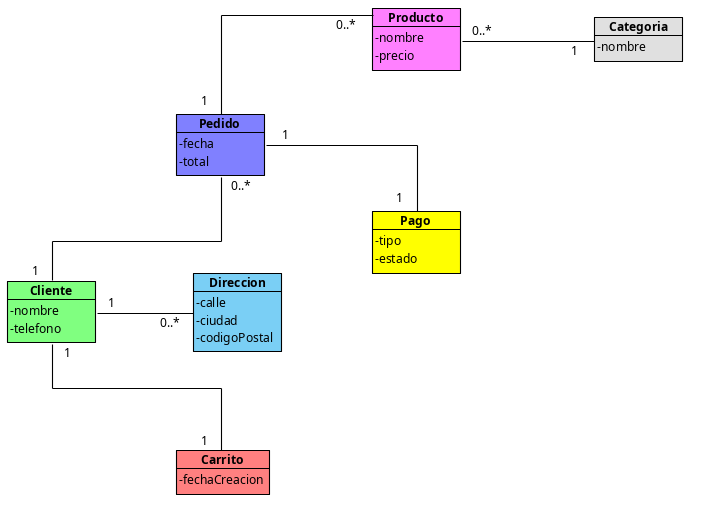
\includegraphics[width=0.85\textwidth]{figs/CasosdeUsoAnalisis.png}
    \caption{Diagrama de clases de análisis del sistema.}
    \label{fig:clases_analisis}
\end{figure}
\clearpage

\subsection{Diagrama de secuencia general del sistema (DSGS)}

La Figura~\ref{fig:dsgs} muestra el \textbf{diagrama de secuencia general del sistema (DSGS)}, 
que representa de forma dinámica las interacciones entre los principales actores externos 
y la \textit{WebApp}. En él se detalla el flujo completo de una compra, 
desde el inicio de sesión del cliente, la selección de productos y la realización del pedido, 
hasta la comunicación con la pasarela de pago \textit{Stripe}
y la notificación del resultado al \textit{bot de Telegram}. 
El diagrama también incluye un flujo alternativo en el que se muestra el manejo de un posible error de pago. 
Este modelo complementa al diagrama de casos de uso al ofrecer una visión temporal del comportamiento global del sistema.

\begin{figure}[H]
    \centering
    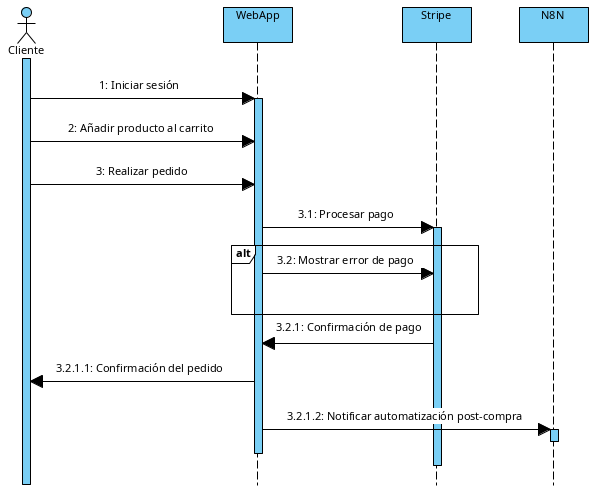
\includegraphics[width=0.9\textwidth]{figs/DSGS.png}
    \caption{Diagrama de secuencia general del sistema (DSGS).}
    \label{fig:dsgs}
\end{figure}
\subsubsection{DSGS-00 Diagrama de secuencia general del sistema}

\begin{table}[H]
\centering
\small
\begin{tabular}{|m{0.28\textwidth}|m{0.65\textwidth}|}
\hline
\textbf{Nombre} & DSGS-00 Diagrama de secuencia general del sistema \\ \hline

\textbf{Actor(es)} & Cliente, WebApp, Stripe, Bot de Telegram \\ \hline

\textbf{Descripción} &
Representa el flujo global del sistema durante el proceso de compra: inicio de sesión del cliente,
gestión del carrito, procesamiento del pago a través de Stripe y notificación del resultado al bot de Telegram,
incluyendo un flujo alternativo en caso de error de pago. \\ \hline

\textbf{Precondiciones} &
El cliente debe tener acceso a la WebApp y existir conexión con Stripe y el bot de Telegram. \\ \hline

\textbf{Postcondiciones} &
El pedido queda confirmado o rechazado, y el bot de Telegram recibe la notificación para ejecutar las tareas automáticas. \\ \hline

\textbf{Flujo principal} &
1. El cliente inicia sesión. \newline
2. Añade productos al carrito. \newline
3. Realiza el pedido. \newline
4. La WebApp envía el pago a Stripe. \newline
5. Stripe confirma el pago. \newline
6. La WebApp confirma el pedido. \newline
7. La WebApp notifica al bot de Telegram para ejecutar tareas post-compra. \\ \hline

\textbf{Flujos alternativos} &
4.a Stripe devuelve un error → la WebApp muestra el fallo al cliente. \\ \hline

\textbf{Requisitos funcionales relacionados} &
RF-01, RF-02, RF-04, RF-06 \\ \hline
\end{tabular}
\caption{Especificación del flujo DSGS-00 — Diagrama de secuencia del sistema.}
\end{table}

\clearpage





\chapter{Diseño}
\input{tex/diseno.tex}

\chapter{Implementación y pruebas}
% Contenidos del capítulo.
% Las secciones presentadas son orientativas y no representan
% necesariamente la organización que debe tener este capítulo.
\section{Implementación}

En este capítulo se describe el proceso de desarrollo de la aplicación, haciendo especial énfasis en los fragmentos de código más representativos del backend. Se han seleccionado tres funciones que ilustran aspectos clave del sistema: la gestión del flujo de compra, la seguridad en la recuperación de contraseñas y la generación de estadísticas para el panel de administración.

\subsection{Creación de pedido}

El método \texttt{crearPedido}, ubicado en \texttt{PedidoController.java}, constituye el núcleo del flujo de compra del sistema. Se ejecuta dentro de una transacción \texttt{@Transactional}, lo que garantiza que, si se produce cualquier error durante el proceso —por ejemplo, stock insuficiente en alguno de los artículos—, todas las operaciones realizadas hasta ese momento se deshacen automáticamente, preservando la integridad de los datos.

Para cada producto del carrito, el sistema verifica la disponibilidad de stock antes de proceder al descuento. El fragmento siguiente muestra esta comprobación, junto con la lógica de actualización del inventario y el disparo automático de la alerta de bajo stock:

\begin{lstlisting}[language=Java, caption={Verificación de stock y notificación al administrador (PedidoController.java).}]
// Verificar stock
if (productoReal.getStock() < item.getCantidad()) {
    throw new RuntimeException(
        "Stock insuficiente para: " + productoReal.getNombre());
}
// Restar stock y persistir
int nuevoStock = productoReal.getStock() - item.getCantidad();
productoReal.setStock(nuevoStock);
productoRepository.save(productoReal);
// Alerta Telegram si stock bajo
if (nuevoStock <= 5) {
    telegramService.notificarStockBajo(
        productoReal.getNombre(), nuevoStock);
}
\end{lstlisting}

Los cálculos monetarios se realizan con \texttt{BigDecimal} en lugar de tipos de coma flotante primitivos, evitando los errores de precisión habituales en operaciones aritméticas con decimales. Una vez completado el proceso, el sistema dispara dos notificaciones externas de forma automática: un correo electrónico de confirmación al cliente y un mensaje al administrador a través del bot de Telegram. Cabe destacar que el estado inicial del pedido depende del método de pago seleccionado: los pagos con Bizum arrancan en estado \texttt{PENDIENTE\_PAGO} hasta que el administrador confirma la transferencia de forma manual.

\subsection{Recuperación de contraseña}

El módulo de recuperación de contraseña, implementado en \texttt{PasswordController.java}, sigue un flujo en dos pasos diseñado con criterios de seguridad. En el primer paso, el sistema genera un token único mediante \texttt{UUID.randomUUID()} y lo almacena en la base de datos junto con una marca de caducidad de una hora. A continuación, envía al usuario un enlace de recuperación por correo electrónico. En el segundo paso, el sistema valida el token recibido, comprueba que no haya expirado y actualiza la contraseña con el nuevo valor proporcionado.

\begin{lstlisting}[language=Java, caption={Generación de token y validación en el reset de contraseña (PasswordController.java).}]
// PASO 1 — Generar token con caducidad de 1 hora
String token = UUID.randomUUID().toString();
usuario.setResetToken(token);
usuario.setTokenExpiration(LocalDateTime.now().plusHours(1));
usuarioRepository.save(usuario);
emailService.sendPasswordResetEmail(email, usuario.getNombre(), token);

// Respuesta ambigua intencionada (evita user enumeration)
return "Si el correo existe, se ha enviado un enlace.";

// PASO 2 — Comprobar caducidad y actualizar contraseña
if (usuario.getTokenExpiration().isBefore(LocalDateTime.now())) {
    return "Error: El enlace ha caducado.";
}
usuario.setPassword(passwordEncoder.encode(newPassword));
usuario.setResetToken(null);
usuario.setTokenExpiration(null);
\end{lstlisting}

Merece especial mención el mensaje de respuesta del primer paso: la formulación \textit{"Si el correo existe, se ha enviado un enlace"} es intencionalmente ambigua. Esta técnica evita la enumeración de usuarios (\textit{user enumeration}), impidiendo que un atacante pueda deducir qué direcciones de correo están registradas en el sistema a partir de las respuestas del servidor. Tras completar el reset, el token se elimina de la base de datos para que no pueda reutilizarse, y la nueva contraseña se almacena hasheada con \textit{BCrypt}, garantizando que nunca se persista en texto plano.

\clearpage
\subsection{Estadísticas del panel de administración}

El endpoint \texttt{getStats}, definido en \texttt{StatsController.java}, centraliza en una única llamada todos los datos que alimentan el dashboard del administrador, consolidando información procedente de cuatro repositorios distintos: pedidos, productos, detalles de pedido y usuarios.

\begin{lstlisting}[language=Java, caption={Cálculo de ingresos y métricas de stock en el panel de administración (StatsController.java).}]
// Ingresos del mes actual vs. mes anterior
LocalDateTime inicioMes =
    LocalDate.now().withDayOfMonth(1).atStartOfDay();
BigDecimal ingresosMes =
    pedidoRepository.sumIngresosPorPeriodo(
        inicioMes, inicioMes.plusMonths(1));
BigDecimal ingresosMesAnterior =
    pedidoRepository.sumIngresosPorPeriodo(
        inicioMes.minusMonths(1), inicioMes);

// Productos con stock crítico
List<Producto> stockCritico =
    productoRepository
        .findByStockLessThanEqualOrderByStockAsc(5);
long sinStock =
    stockCritico.stream()
        .filter(p -> p.getStock() == 0).count();

// Top 5 productos más vendidos
for (Object[] row : detallePedidoRepository
        .findTopProductos(PageRequest.of(0, 5))) { ... }
\end{lstlisting}

La comparativa de ingresos entre el mes actual y el mes anterior permite al administrador detectar tendencias de ventas de forma inmediata. El cálculo excluye los pedidos cancelados y los pendientes de pago, de modo que el valor mostrado refleja únicamente ingresos reales confirmados. En cuanto al inventario, el panel diferencia entre productos sin stock (\texttt{stock = 0}) y productos con stock bajo (\texttt{stock} $\leq$ \texttt{5}), proporcionando dos niveles de alerta independientes. El listado de los cinco productos más vendidos se obtiene mediante una consulta JPQL con agregación y paginación controlada con \texttt{PageRequest}, limitando el resultado a los primeros cinco registros.


\section{Pruebas funcionales}


\section{Pruebas de rendimiento}


\section{Pruebas de usabilidad}

\chapter{Conclusiones}
% Contenidos del capítulo.
% Las secciones presentadas son orientativas y no representan
% necesariamente la organización que debe tener este capítulo.

\section{Revisión de costes}

En este apartado se revisan los costes reales del proyecto y se comparan con las estimaciones realizadas en la fase de planificación, recogidas en el Capítulo~3.

En cuanto a los \textbf{costes de software}, el resultado ha sido idéntico al estimado: todas las herramientas empleadas durante el desarrollo —Angular, Spring Boot, MySQL, Visual Studio Code, Postman y Visual Paradigm con licencia académica— son gratuitas, por lo que el coste final en este concepto ha sido de \textbf{0~€}, tal y como se preveía.

Respecto a los \textbf{costes de hardware}, el portátil personal utilizado durante el desarrollo tenía un valor de 1.200~€ y se amortizó a lo largo de cuatro meses de desarrollo efectivo, sobre una vida útil estimada de cuatro años, lo que supone un coste imputado de \textbf{100~€}, coincidiendo con la estimación inicial.

En lo relativo a los \textbf{costes indirectos} —electricidad, conexión a internet y otros gastos asociados al uso del equipo durante el desarrollo—, el importe final se estima en \textbf{80~€}, en línea con lo planificado.

En cuanto a los \textbf{costes de personal}, la distribución del trabajo entre los distintos perfiles definidos en la planificación —jefe de proyecto, desarrollador \textit{backend}, desarrollador \textit{frontend} y \textit{tester}— se ha ajustado en términos generales a las horas estimadas, si bien la fase de integración y pruebas requirió una dedicación algo superior a la prevista inicialmente. No obstante, dado que el proyecto ha sido desarrollado en su totalidad por una sola persona en el contexto de un TFG, sin retribución económica real, este desvío no ha supuesto un impacto en el presupuesto efectivo.

En consecuencia, el \textbf{coste total estimado del proyecto} asciende a \textbf{5.380~€}, sin variaciones significativas respecto a la planificación original. La utilización exclusiva de herramientas gratuitas y de código abierto ha sido el factor clave para mantener el presupuesto dentro de los márgenes previstos, confirmando la viabilidad económica del proyecto expuesta en el Capítulo~3.

\section{Conclusiones}

El presente proyecto ha permitido desarrollar una tienda online completa y funcional para la Droguería Mercería Inés, cubriendo desde el catálogo de productos y el proceso de compra con pasarela de pago hasta el panel de administración y el sistema de notificaciones. A continuación se revisa el grado de cumplimiento de cada uno de los objetivos planteados al inicio del trabajo.

El \textbf{objetivo principal} —desarrollar una tienda online funcional que permita a los clientes consultar el catálogo, realizar pedidos y efectuar pagos de forma segura— se ha alcanzado en su totalidad. La aplicación implementa el flujo completo de compra, desde el registro del usuario hasta la confirmación del pedido con generación automática de factura en PDF.

Respecto a los \textbf{objetivos secundarios}, todos han sido alcanzados satisfactoriamente:

\begin{itemize}
    \item La plataforma web propia proporciona al negocio una presencia digital independiente de las redes sociales, con un catálogo consultable en cualquier momento y desde cualquier dispositivo.
    \item La propietaria dispone de un panel de administración desde el que puede gestionar el inventario, actualizar productos con imágenes almacenadas en Cloudinary y hacer seguimiento de los pedidos recibidos.
    \item El bot de Telegram notifica automáticamente al administrador ante cada nueva compra y emite alertas cuando el stock de un producto desciende por debajo del umbral configurado.
    \item El desarrollo con \textbf{Angular} y \textbf{Spring Boot} ha proporcionado una base sólida en las tecnologías empleadas en las prácticas profesionales en \textbf{Capgemini}, resultando de aplicación directa en el entorno laboral.
    \item La solución se ha construido íntegramente con herramientas gratuitas y de código abierto, demostrando que es posible desarrollar un sistema de comercio electrónico profesional sin incurrir en costes de licencias.
\end{itemize}

Entre los aspectos que han supuesto un mayor reto técnico destaca la integración del \textbf{bot de Telegram}. Al tratarse de una tecnología no trabajada previamente, requirió un proceso de aprendizaje específico: primero comprendiendo el protocolo de la API de Telegram y posteriormente implementando el sistema de polling manual con \texttt{RestTemplate} para la recepción de comandos y el envío de notificaciones.

A nivel de aprendizaje, este proyecto ha consolidado el conocimiento de la arquitectura cliente-servidor mediante una aplicación real y completa, abarcando tanto el frontend en Angular como el backend en Spring Boot, con toda la integración que ello implica: autenticación JWT, gestión transaccional, pasarela de pago y servicios externos.

Por último, cabe señalar que la propietaria del negocio ha podido ver y probar la aplicación, valorando positivamente tanto el panel de administración como la experiencia de compra. El despliegue en un servidor público queda como trabajo futuro pendiente de acuerdo con sus necesidades y disponibilidad.

\section{Trabajo futuro}

Aunque el sistema desarrollado cubre todos los requisitos funcionales planteados, durante el proceso de desarrollo y las pruebas realizadas se han identificado varias líneas de mejora que podrían abordarse en versiones futuras de la aplicación.

\begin{itemize}
    \item \textbf{Despliegue en producción.} La aplicación está preparada para ser desplegada en un servidor público, pero actualmente solo funciona en entorno local. El siguiente paso natural es publicarla en una plataforma de alojamiento en la nube para que sea accesible a cualquier cliente desde internet.

    \item \textbf{Adaptación para dispositivos móviles.} Aunque la interfaz es funcional en escritorio, una adaptación específica del diseño para teléfonos y tabletas mejoraría significativamente la experiencia de los clientes que acceden desde dispositivos móviles.

    \item \textbf{Integración con servicios de mensajería y envío.} Actualmente el sistema gestiona el pedido y el pago, pero la logística de envío queda fuera del alcance de la aplicación. Integrar un servicio de mensajería permitiría generar etiquetas de envío, comunicar el estado del transporte al cliente y cerrar el ciclo completo de la compra online.

    \item \textbf{Sistema de reseñas de productos.} Permitir que los clientes que hayan adquirido un producto dejen una valoración y un comentario aportaría información útil tanto a otros compradores como a la propietaria para conocer la satisfacción con el catálogo.

    \item \textbf{Procesamiento asíncrono en la creación de pedidos.} Como se observó en las pruebas de rendimiento, el endpoint \texttt{POST /api/pedidos/crear} tarda 1.870 ms debido a que el envío del correo de confirmación y la notificación de Telegram se realizan de forma síncrona. Procesarlas de forma asíncrona, por ejemplo mediante \texttt{@Async} de Spring, reduciría el tiempo de respuesta percibido por el usuario.

    \item \textbf{Mejora de la usabilidad en el proceso de pago.} Las pruebas de usabilidad evidenciaron que el formulario de \textit{checkout} genera cierta fricción en perfiles con escasa experiencia en compras online. Incorporar indicaciones contextuales y mensajes de ayuda en ese paso haría la experiencia más accesible para ese tipo de usuarios.
\end{itemize}




%\pagestyle{appendix}

%\appendix
%\chapter{Apéndice}
%\input{tex/apendice.tex}

\addcontentsline{toc}{chapter}{Bibliografía}
\bibliographystyle{unsrt}
\bibliography{bib/bibliografia}




\end{document}

%%% Local Variables:
%%% mode: latex
%%% TeX-master: t
%%% End:
